%%%%%%%%%%%%%%%%%%%%%%%%%%%%%%%%%%%%%%%%%
% Sullivan Business Report
% LaTeX Template
% Version 1.0 (May 5, 2022)
%
% This template originates from:
% https://www.LaTeXTemplates.com
%
% Author:
% Vel (vel@latextemplates.com)
%
% License:
% CC BY-NC-SA 4.0 (https://creativecommons.org/licenses/by-nc-sa/4.0/)
%
%%%%%%%%%%%%%%%%%%%%%%%%%%%%%%%%%%%%%%%%%

%----------------------------------------------------------------------------------------
%	CLASS, PACKAGES AND OTHER DOCUMENT CONFIGURATIONS
%----------------------------------------------------------------------------------------

\documentclass[
	a4paper, % Paper size, use either a4paper or letterpaper
	12pt, % Default font size, the template is designed to look good at 12pt so it's best not to change this
	%unnumberedsections, % Uncomment for no section numbering
]{CSSullivanBusinessReport}

\addbibresource{sample.bib} % BibLaTeX bibliography file

%----------------------------------------------------------------------------------------
%	REPORT INFORMATION
%----------------------------------------------------------------------------------------

\reporttitle{Data analysis} % The report title to appear on the title page and page headers, do not create manual new lines here as this will carry over to page headers

\reportsubtitle{Analysis of rooftiles\\ Image dataset visualization and preprocessing} % Report subtitle, include new lines if needed

\reportauthors{Created by:\\\smallskip Christian Wanschers \\ Sara Eftekhar Azam \\ Bastiaan Verheul \\ Nino van Alphen } % Report authors/group/department, include new lines if needed

\reportdate{\today} % Report date, include new lines for additional information if needed

\rightheadercontent{
\includegraphics[width=2cm]{inhollandlogo.pdf}} % The content in the right header, you may want to add your own company logo or use your company/department name or leave this command empty for no right header content

%----------------------------------------------------------------------------------------

\begin{document}

%----------------------------------------------------------------------------------------
%	TITLE PAGE
%----------------------------------------------------------------------------------------

\thispagestyle{empty} % Suppress headers and footers on this page

\begin{fullwidth} % Use the whole page width
	\vspace*{-0.075\textheight} % Pull logo into the top margin
	
	\hfill
\includegraphics[width=5cm]{inhollandlogo.pdf} % Company logo

	\vspace{0.15\textheight} % Vertical whitespace

	\parbox{0.9\fulltextwidth}{\fontsize{50pt}{52pt}\selectfont\raggedright\textbf{\reporttitle}\par} % Report title, intentionally at less than full width for nice wrapping. Adjust the width of the \parbox and the font size as needed for your title to look good.
	
	\vspace{0.03\textheight} % Vertical whitespace
	
	{\LARGE\textit{\textbf{\reportsubtitle}}\par} % Subtitle
	
	\vfill % Vertical whitespace
	
	{\Large\reportauthors\par} % Report authors, group or department
	
	\vfill\vfill\vfill % Vertical whitespace
	
	{\large\reportdate\par} % Report date
\end{fullwidth}

\newpage

%----------------------------------------------------------------------------------------
%	DISCLAIMER/COPYRIGHT PAGE
%----------------------------------------------------------------------------------------

\thispagestyle{empty} % Suppress headers and footers on this page

% \begin{twothirdswidth} % Content in this environment to be at two-thirds of the whole page width
% 	\footnotesize % Reduce font size
	
% 	\subsection*{Disclaimer}

% 	Lorem ipsum dolor sit amet, consectetur adipiscing elit. Praesent porttitor arcu luctus, imperdiet urna iaculis, mattis eros. Pellentesque iaculis odio vel nisl ullamcorper, nec faucibus ipsum molestie. Sed dictum nisl non aliquet porttitor. Etiam vulputate arcu dignissim, finibus sem et, viverra nisl. Aenean luctus congue massa, ut laoreet metus ornare in. Nunc fermentum nisi imperdiet lectus tincidunt vestibulum at ac elit.
	
% 	\subsection*{Copyright}
	
% 	\textcopyright~[Year] [Company] 
	
% 	Copyright notice text\ldots In hac habitasse platea dictumst. Curabitur mattis elit sit amet justo luctus vestibulum. In hac habitasse platea dictumst. Pellentesque lobortis justo enim, a condimentum massa tempor eu. Ut quis nulla a quam pretium eleifend nec eu nisl. Nam cursus porttitor eros, sed luctus ligula convallis quis.
	
% 	\subsection*{Contact}
	
% 	Address Line 1\\
% 	Address Line 2\\
% 	Address Line 3
	
% 	Business Number 123456
	
% 	Contact: name@company.com
	
% 	\vfill % Push the following down to the bottom of the page
	
% 	\subsubsection*{Changelog}
	
% 	\scriptsize % Reduce font size further
	
% 	\begin{tabular}{@{} L{0.05\linewidth} L{0.15\linewidth} L{0.6\linewidth} @{}} % Column widths specified here, change as needed for your content
% 		\toprule
% 		v1.0 & 20XX-02-05 & Lorem ipsum dolor sit amet, consectetur adipiscing elit. Praesent porttitor arcu luctus, imperdiet urna iaculis, mattis eros.\\
% 		v1.1 & 20XX-02-27 & Pellentesque iaculis odio vel nisl ullamcorper, nec faucibus ipsum molestie.\\
% 		v1.2 & 20XX-03-15 & Sed dictum nisl non aliquet porttitor.\\
% 		\bottomrule
% 	\end{tabular}
% \end{twothirdswidth}

\newpage

%----------------------------------------------------------------------------------------
%	TABLE OF CONTENTS
%----------------------------------------------------------------------------------------

\begin{twothirdswidth} % Content in this environment to be at two-thirds of the whole page width
	\tableofcontents % Output the table of contents, automatically generated from the section commands used in the document
\end{twothirdswidth}

\newpage

%----------------------------------------------------------------------------------------
%	SECTIONS
%----------------------------------------------------------------------------------------

\section{The dataset}
\begin{fullwidth}
	The dataset we will be discussing in this report is an image based dataset from our client Tilmann Köster. 
	In the dataset, which he made himself, is populated with around 7800 images of rooftile. 
	The dataset has both front and back images of all rooftiles in roughly equal amounts. 
	The dataset is already annotated. The annotations are documented by the client and given to us. 

	\begin{itemize}
		\item All rooftiles are within their own folder called (for example) \verb|d0000_b_blw_g_OVH|.
		\item \verb|d0000| is the number of the rooftile, it is assumed by the client that no more than 9999 different kinds of rooftiles will ever be included.
		\item \verb|b| is means the side (in Dutch) of the rooftile. \verb|b| is the topside, \verb|o| is the bottomside.
		\item \verb|blw| is the colour code of the rooftile. See table \ref{tab:abbr_colours} for all possible options.
		\item \verb|g| or \verb|n| means gebruikt (used) or nieuw (new).
		\item \verb|OVH| is the abbreviation of the name of the rooftile. See table \ref{tab:abbr_rooftile_names} for all possible names.
	\end{itemize}
\end{fullwidth}

\begin{table}[H]
    \begin{tabular}{lll}
        \textbf{Abbr.}        & \textbf{NL}         & \textbf{EN}                  \\
        blw          & Blauw      & blue                \\
        nrd          & natuurrood & nature red          \\
        ord          & oranjerood & orange red          \\
        mzv          & matzwart   & vitrified mattblack \\
        zw           & zwart      & black               \\
        rb           & rood bruin & Red Brown          
    \end{tabular}
    \caption{Abbreviations for colors}
    \label{tab:abbr_colours}
\end{table}

\begin{table}[H]
    \begin{tabular}{lll}
        \textbf{Abbr.}        & \textbf{Name} \\
        \verb|OVH|  & Opnieuw Verbeterde Holle \\
        \verb|TDN44|    & Tuile de Nord 44 \\
        \verb|VH|   & Verbeterde Holle  \\
        \verb|NS|   & Nelskamp Sigma \\
        \verb|OVHvario| & Opnieuw Verbeterde Holle vario \\
        \verb|OVH200|   & Opnieuw Verbeterde Holle 200 \\
        \verb|OH|   & Oude Holle \\
        \verb|VHm6| & Verbeterde Holle Monier 6 \\
        \verb|VHvOord|  & Verbeterde Holle van Oord \\
        \verb|VHO&|  &  Verbeterde Holle O\&Z \\
        \verb|NSSP| & Nelskamp S-Pfanne \\
        \verb|RBBS| & RBB Sneldek
    \end{tabular}
    \caption{Abbreviations for rooftile names}
    \label{tab:abbr_rooftile_names}
\end{table}
\newpage
\section{Visualizations of Dataset}
First, it is important to analyze and visualize the properties of the original images. 
We did this with the following steps\dots

\subsection{BGR channels of original dataset}
\sidenote{We needed to analyze the color distribution of the colors to understand the average colors used within the dataset. 
The figure below shows the result of this analysis for the whole dataset and below that examples of 3 random images and their own color channels.}

\begin{figure}[H] % [H] forces the figure to be output where it is defined in the code (it suppresses floating)
	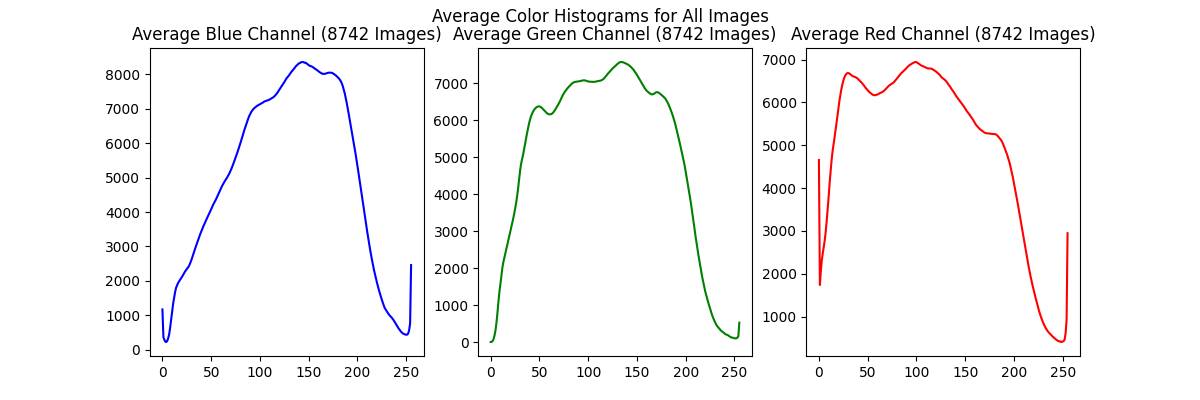
\includegraphics[width=\linewidth]{average_color_histogram.png}
	\caption{Average colors as colorchannels.}
	\label{fig:average_color_histogram} % Label for referencing this figure in the text automatically
\end{figure}

\begin{figure}[H] % [H] forces the figure to be output where it is defined in the code (it suppresses floating)
	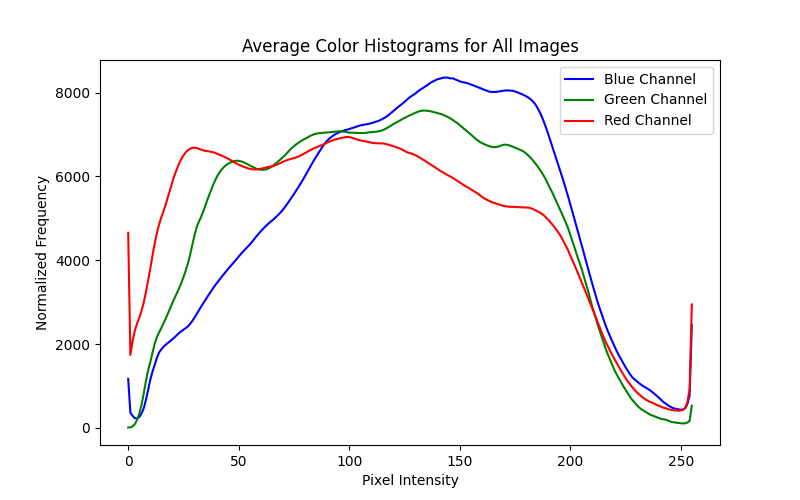
\includegraphics[width=\linewidth]{average_color_histogram_overlap_full.png}
	\caption{Overlapping colors as colorchannels.}
	\label{fig:average_color_histogram_overlap_full} % Label for referencing this figure in the text automatically
\end{figure}

\newpage
\subsection{Visualizing aspect ratios}
\sidenote[][]{We also need to check the aspect ratios to check whether non-square images were present in our dataset. And as you can see, not all have a square aspect ratio. However, this is required for most and simpler YOLO algorithms}

\begin{figure}[H] % [H] forces the figure to be output where it is defined in the code (it suppresses floating)
	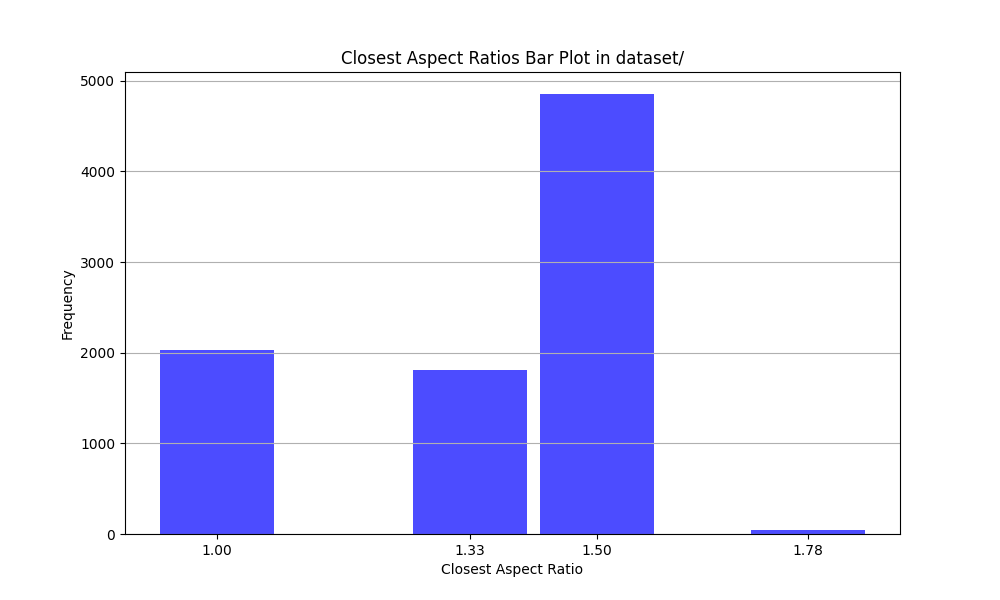
\includegraphics[width=\linewidth]{aspect_ratio_result.png}
	\caption{Aspect ratios.}
	\label{fig:aspect_ratio_result} % Label for referencing this figure in the text automatically
\end{figure}

\newpage
\subsection{Visualizing resolutions}
\begin{fullwidth} % Use the whole page width
Before changing the properties of the images, 
we also need to check the resolutions to determine if we can safely decrease it to make it easier to work with the model without long loading times which comes with using big files. 
All images in the dataset we got from the client had roughly had a 4K resolution, which meant each image was around 4- to 6MB in size. 
This meant the total dataset was around 75GB for 7800 images. 
The size means that the dataset is difficult to process in code and the model generally does not require images with a resolution that large. 
We decided to scale the images down when the resolution was of a higher value than 3000 in either width or length. 
This meant a file size decrease of about 94\%. 
This resulted in the total size of the dataset decreasing to less than 4GB and thus being much easier to process. 
The figure below shows the result resolution rescaling.
\end{fullwidth} % End of use the whole page width

\sidenote{Rescaling was done immediatly since the 8742 images within the dataset resulted in a size of over 75GB which isn't easy to work with.}
\begin{figure}[H] % [H] forces the figure to be output where it is defined in the code (it suppresses floating)
	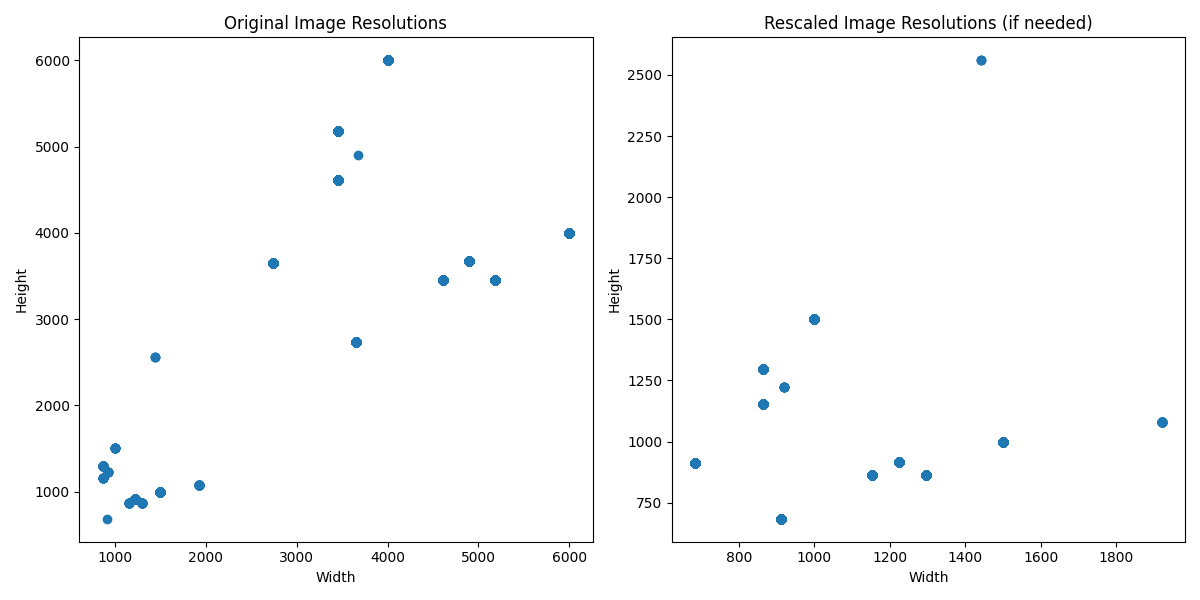
\includegraphics[width=\linewidth]{rescale_res_result.png}
	\caption{Resolutions of images before \& after}
	\label{fig:rescale_res_result} % Label for referencing this figure in the text automatically
\end{figure}

% \begin{marginfigure} % Use the marginfigure environment for figures to be output to the margin
% 	
\includegraphics[width=\linewidth]{placeholder.jpg}
% 	\caption{Margin figure caption.}
% \end{marginfigure}

% \begin{marginfigure} % Use the marginfigure environment for figures to be output to the margin
% 	
\includegraphics[width=\linewidth]{placeholder.jpg}
% 	\caption{Margin figure caption.}
% \end{marginfigure}
\newpage

\section{Changes to Dataset} % Top level section
\begin{fullwidth}We need to change some properties to prepare the dataset before feeding it to a model\dots\end{fullwidth}

\subsection{Updates to resolution}
\begin{fullwidth}As we mentioned earlier, we decreased the resolution of all images in the whole dataset to make it more manageable. \end{fullwidth}
See \ref{fig:rescale_res_result}.

\subsection{File extension formatting}
\begin{fullwidth}
Most images were of .JPG format and some of .JPEG and .PNG format. To make all these images the same file format we chose to convert them all to the PNG format. 
\end{fullwidth}

\subsection{Applying grayscale}
\sidenote{We need to apply a grayscale effect to remove the BGR-channels currently present in the image. 
The image contains colours which might interfere with classification and makes it harder to bring out the details.
Applying Grayscale makes sure those details are easier to bring out in the next preprocessing techniques.}
\begin{figure}[H] % [H] forces the figure to be output where it is defined in the code (it suppresses floating)
	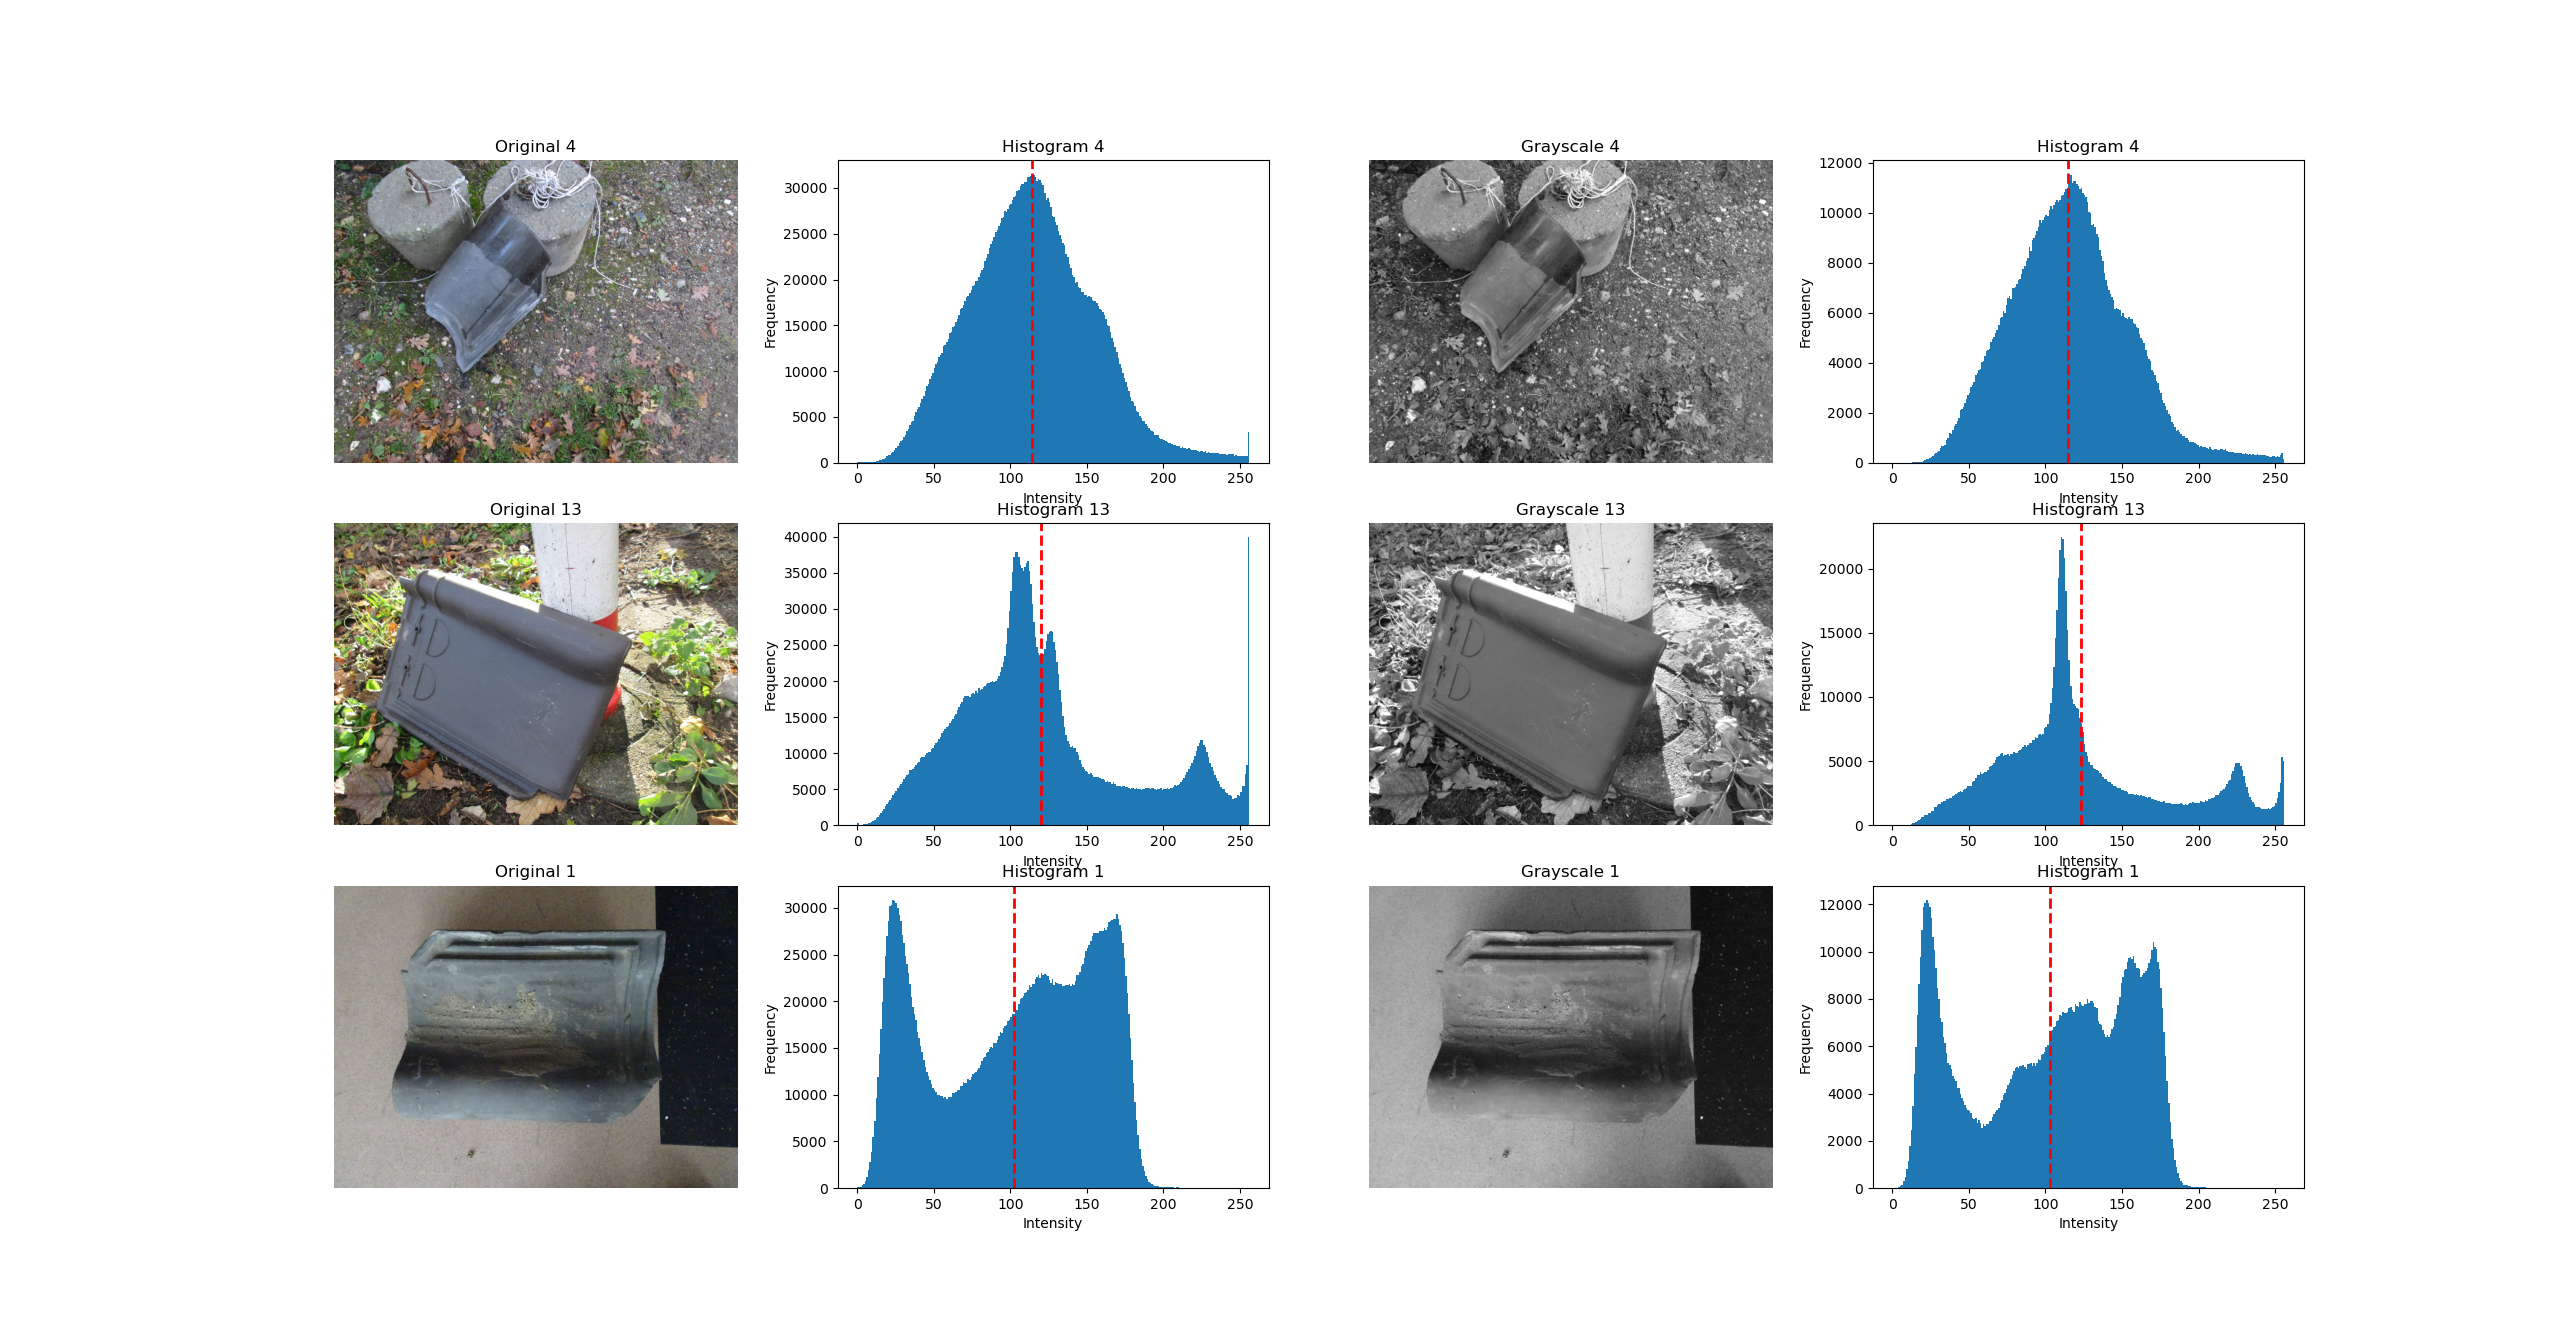
\includegraphics[width=\linewidth]{grayscale_graph_histogram.png}
	\caption{Grayscale of images plot}
	\label{fig:grayscale_graph_histogram} % Label for referencing this figure in the text automatically
\end{figure}

\newpage
\subsection{Applying normalization}
\sidenote[][1cm]{After grayscaling, normalization needs to be applied to normalize contrast. 
Doing this removes some glare or extreme lighting effects caused by the camera lens.}
\begin{figure}[H] % [H] forces the figure to be output where it is defined in the code (it suppresses floating)
	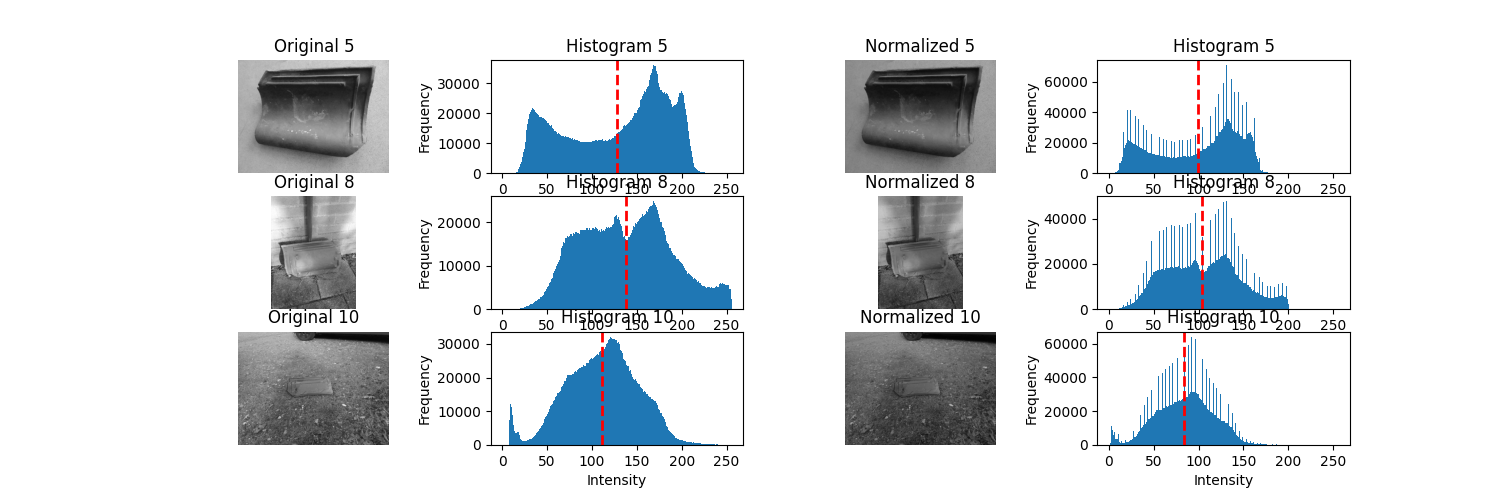
\includegraphics[width=\linewidth]{normalization_conversion_before_after.png}
	\caption{Normalization of images plot}
	\label{fig:normalization_conversion_before_after} % Label for referencing this figure in the text automatically
\end{figure}

% \newpage
\subsection{Applying CLAHE}
\sidenote{Lastly, CLAHE is applied to bring out more details. 
CLAHE does this to dampen some of the higher pixel values and placing them below the average threshold, 
so that details appear more sharp.}
\begin{figure}[H] % [H] forces the figure to be output where it is defined in the code (it suppresses floating)
	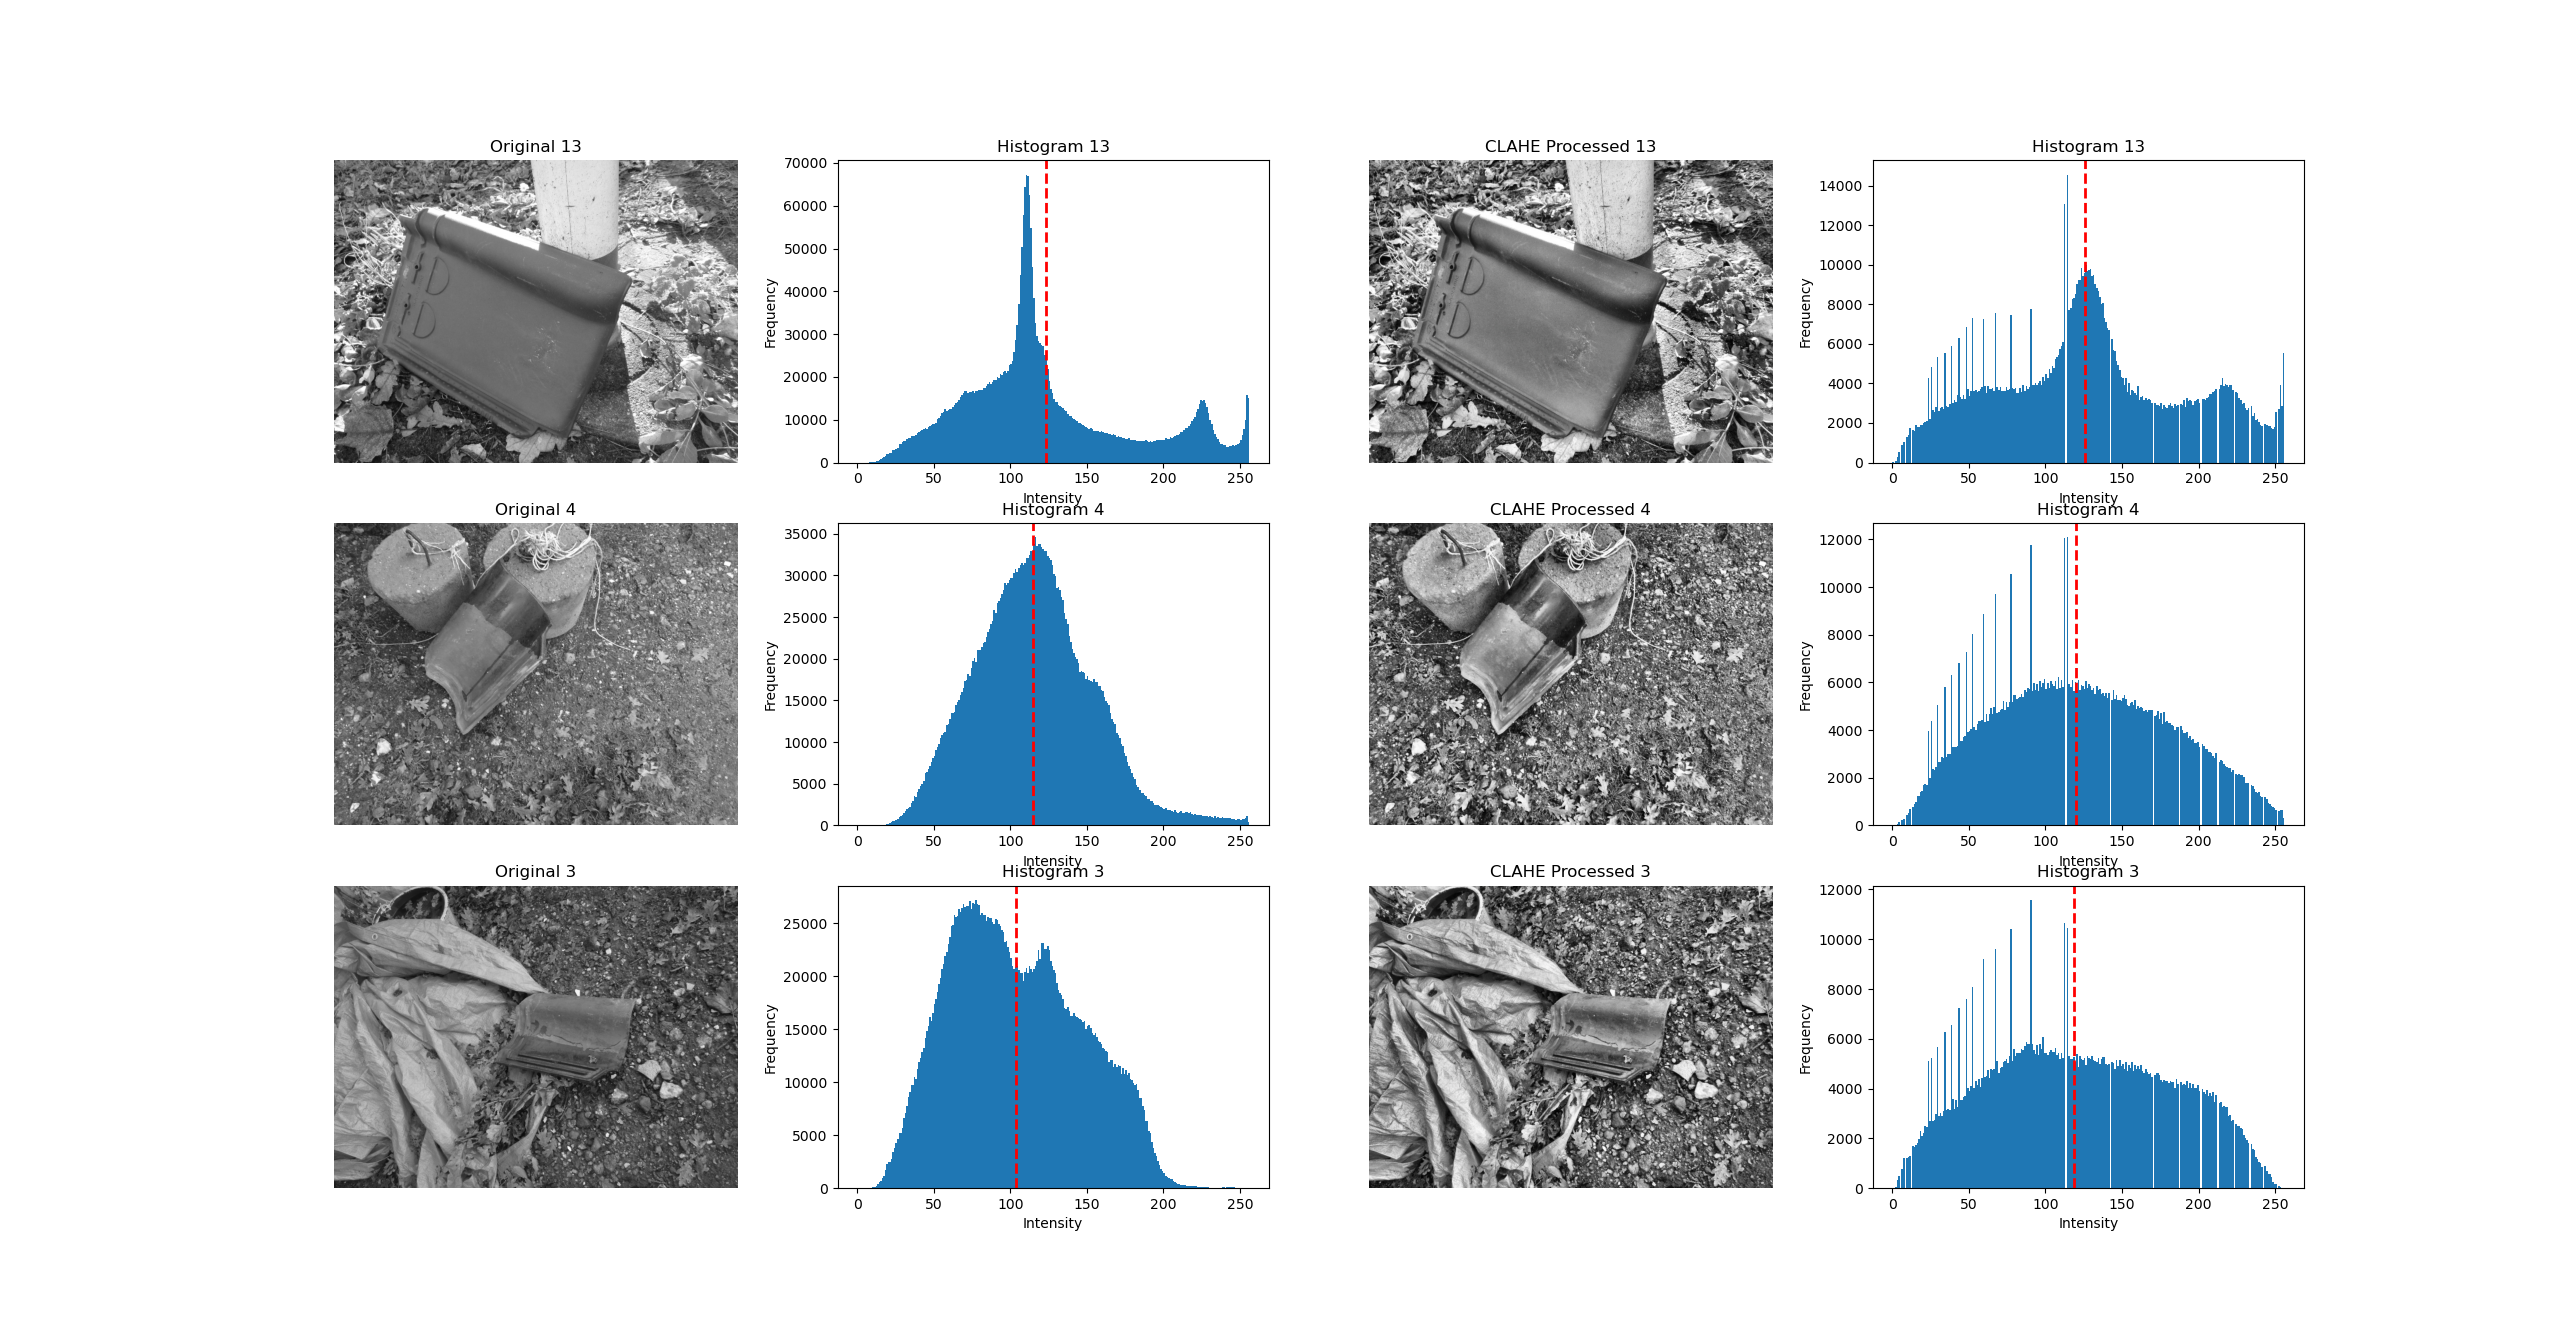
\includegraphics[width=\linewidth]{clahe_graph_histogram.png}
	\caption{CLAHE of images plot}
	\label{fig:clahe_graph_histogram} % Label for referencing this figure in the text automatically
\end{figure}
\newpage
\subsection{Splitting data based on side of rooftile}
The dataset consists of 2 types of images per rooftile:
\begin{itemize}
	\item Picture from the top
	\item Picture from the bottom
\end{itemize}

\sidenote{As described in the first section, all folders are on the same level. This means that top and bottom images are on the same directory level as well. 
We don't want that. What we want is to split the folders based on the top/bottom side of the rooftile so we can train two models, one for each.
We end up with the following folderstructure (Not that this does not include all folders):}

\begin{forest}
	for tree={
		font=\ttfamily,
		grow'=0,
		child anchor=west,
		parent anchor=south,
		anchor=west,
		calign=first,
		edge path={
			\noexpand\path [draw, \forestoption{edge}]
			(!u.south west) +(7.5pt,0) |- node[fill,inner sep=1.25pt] {} (.child anchor)\forestoption{edge label};
		},
		before typesetting nodes={
			if n=1
			{insert before={[,phantom]}}
			{}
		},
		fit=band,
		before computing xy={l=15pt},
	}
	[dataset
		[b
			[d0000\_b\_blw\_g\_OVH
				[d0000\_b\_blw\_g\_OVH (1).png]
				[d0000\_b\_blw\_g\_OVH (2).png]
				[d0000\_b\_blw\_g\_OVH (3).png]
			]
			[d0001\_b\_blw\_n\_TDN44
				[d0001\_b\_blw\_n\_TDN44 (1).png]
				[d0001\_b\_blw\_n\_TDN44 (2).png]
				[d0001\_b\_blw\_n\_TDN44 (3).png]
			]
		]
		[o
			[d0000\_o\_blw\_g\_OVH
				[d0000\_o\_blw\_g\_OVH (1).png]
				[d0000\_o\_blw\_g\_OVH (2).png]
				[d0000\_o\_blw\_g\_OVH (3).png]
			]
			[d0001\_o\_blw\_n\_TDN44
				[d0001\_o\_blw\_n\_TDN44 (1).png]
				[d0001\_o\_blw\_n\_TDN44 (2).png]
				[d0001\_o\_blw\_n\_TDN44 (3).png]
			]
		]
	]
\end{forest}

\subsection{Training and testing data}

\begin{fullwidth}
	After splitting the top and bottom side of the rooftiles we will split the data into training and testing but there is a small catch: we want to keep the proportion of the different rooftiles within each set.
	To do this we will use stratified splitting.
	This is so we don't dont end up with a lot of one type of rooftile and a lot less of another type in either training or testing set. 
	A training ratio of 70\% will be used as default ratio. We will use \verb|train_test_split| from Python's library \verb|sklearn| for splitting into training and testing.
\end{fullwidth}

\sidenote{By doing stratified splitting, we end up with the following folderstructure:}

\begin{forest}
    for tree={
        font=\ttfamily\scriptsize,
        grow'=0,
        child anchor=west,
        parent anchor=south,
        anchor=west,
        calign=first,
        edge path={
            \noexpand\path [draw, \forestoption{edge}]
            (!u.south west) +(7.5pt,0) |- node[fill,inner sep=1.25pt] {} (.child anchor)\forestoption{edge label};
        },
        before typesetting nodes={
            if n=1
            {insert before={[,phantom]}}
            {}
        },
        fit=band,
        before computing xy={l=15pt},
        s sep=2pt, % Adjust vertical spacing
    },
	scale=0.1,
    [dataset
        [test
            [b
                [d0000\_b\_blw\_g\_OVH
                    [d0000\_b\_blw\_g\_OVH (1).png]
                    [d0000\_b\_blw\_g\_OVH (2).png]
                ]
                [d0001\_b\_blw\_n\_TDN44
                    [d0001\_b\_blw\_n\_TDN44 (1).png]
                    [d0001\_b\_blw\_n\_TDN44 (2).png]
                ]
            ]
            [o
                [d0000\_o\_blw\_g\_OVH
                    [d0000\_o\_blw\_g\_OVH (1).png]
                    [d0000\_o\_blw\_g\_OVH (2).png]
                ]
                [d0001\_o\_blw\_n\_TDN44
                    [d0001\_o\_blw\_n\_TDN44 (1).png]
                    [d0001\_o\_blw\_n\_TDN44 (2).png]
                ]
            ]
        ]
        [train
            [b
                [d0000\_b\_blw\_g\_OVH
                    [d0000\_b\_blw\_g\_OVH (1).png]
                    [d0000\_b\_blw\_g\_OVH (2).png]
                ]
                [d0001\_b\_blw\_n\_TDN44
                    [d0001\_b\_blw\_n\_TDN44 (1).png]
                    [d0001\_b\_blw\_n\_TDN44 (2).png]
                ]
            ]
            [o
                [d0000\_o\_blw\_g\_OVH
                    [d0000\_o\_blw\_g\_OVH (1).png]
                    [d0000\_o\_blw\_g\_OVH (2).png]
                ]
                [d0001\_o\_blw\_n\_TDN44
                    [d0001\_o\_blw\_n\_TDN44 (1).png]
                    [d0001\_o\_blw\_n\_TDN44 (2).png]
                ]
            ]
        ]
    ]
\end{forest}

% \subsubsection{Training}

% \subsubsection{Testing}

\newpage
\subsection{Image resizing}
Since most image recognition models require the images in the dataset to be of square format, and most images in our dataset are not square, we need to come up with a technique to make non-square images square. First, we will resize images to the target resolution of 640 by 640.
\begin{marginfigure} % Use the marginfigure environment for figures to be output to the margin
	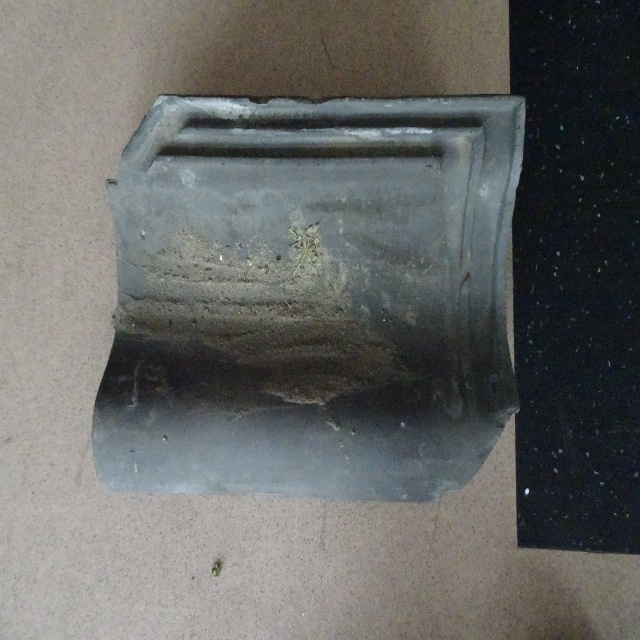
\includegraphics[width=\linewidth]{square_dataset/square0.JPG}
	\caption{An example of resized image that is streched.}
\end{marginfigure}

However, simply resizing images to the target size is not sufficient since images in the dataset are not square. Simply resizing images will make resized images streched, which might be harmful in training the model.

\begin{marginfigure} % Use the marginfigure environment for figures to be output to the margin
	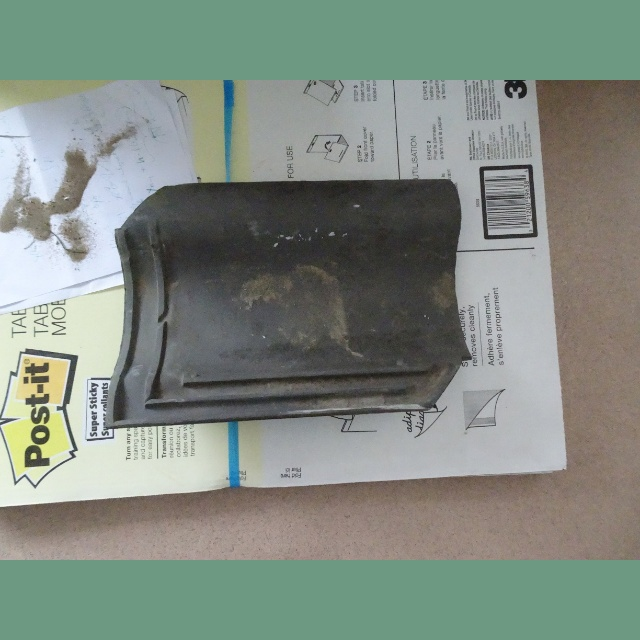
\includegraphics[width=\linewidth]{square_dataset/square1.JPG}
	\caption{An example of horizontal resized image.}
\end{marginfigure}

To convert none square images to square images, we add background to the images. This is done by placing padding with a random color around the image to fill up the blank space required to make it square.
Depending on whether the original image is vertical or horizontal, we add vertical padding or horizontal padding so that the final image becomes square.


\begin{marginfigure} % Use the marginfigure environment for figures to be output to the margin
	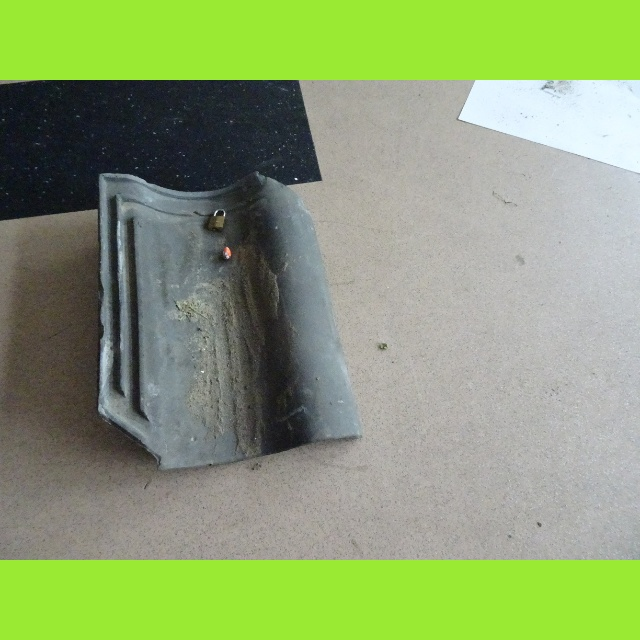
\includegraphics[width=\linewidth]{square_dataset/square2.JPG}
	\caption{Example of resized image.}
\end{marginfigure}

We could simply add a black background to all images but to make sure adding single color background does not add bias to images, we have used random color for the background. 
In the code, the target resolution is 640*640 pixels. This resolution is required by most YOLO-models which could be used as the main algorithm classifying the rooftiles. However, the implemntation of code is genral and can be used for any target resolution. 
To the side are a few examples of images converted to a square aspect ratio.


\begin{marginfigure} % Use the marginfigure environment for figures to be output to the margin
	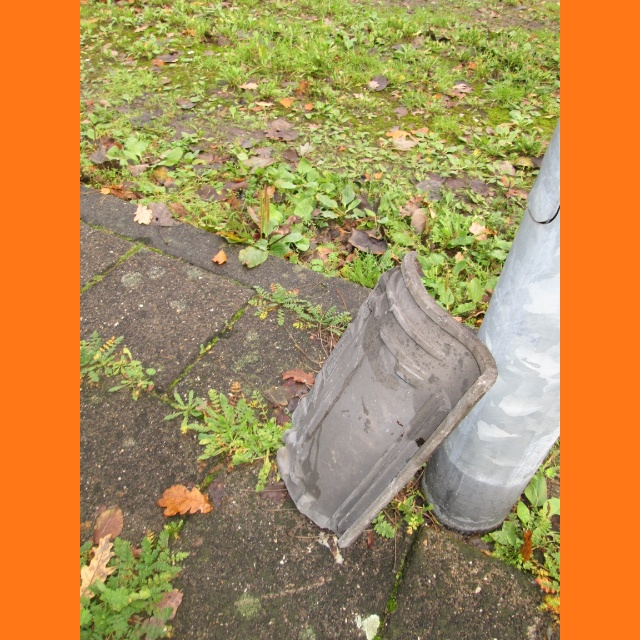
\includegraphics[width=\linewidth]{square_dataset/square3.JPG}
	\caption{Example of vertical image.}
\end{marginfigure}

To explain how the resizing is done, consider the following example: a 1800 by 1200 image that we want to convert to 600 by 600 image (number are chosen for simplicity). To make 1800 by 1200 into 600 by 600 square, first we have to resize it by a factor of 1/3 (it is the minimum of 600/1800 = 1/3 and 600/1200 = 1/2). After resizing the original image by a factor of 1/3, we get to a 600 by 400 image. To make this image square, we need to add 100 pixels of padding to each side of this resized image to get a 600 by 600 image.


% \begin{marginfigure} % Use the marginfigure environment for figures to be output to the margin
% 	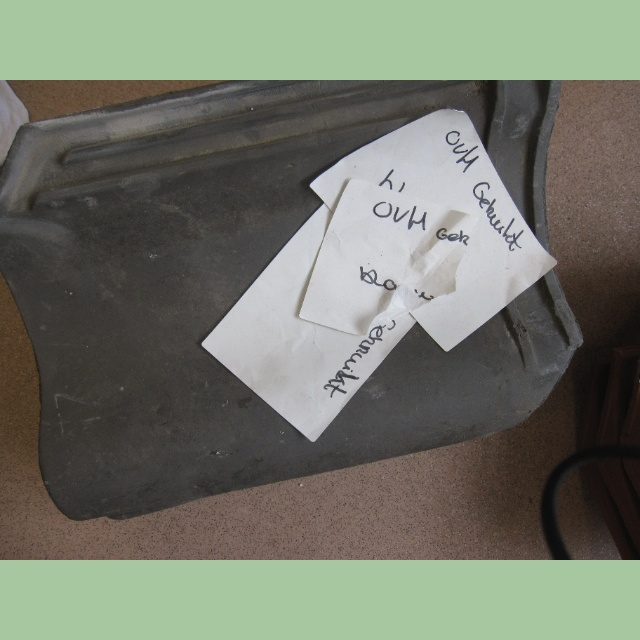
\includegraphics[width=\linewidth]{square_dataset/square5.JPG}
% 	\caption{Square5}
% \end{marginfigure}

\newpage
\subsection{Data augmentation}
\begin{fullwidth}
A few augmentation techniques are applied to artificially increase the dataset and training data. 
It's important to realize that this is just done for training and not testing, 
since testing requires the images to be as closely to the real world as possible. 
The primary goal of data augmentation is to increase the diversity of the training dataset. 
Below are a few simple techniques which can be applied to any image in the dataset:
\end{fullwidth}

% \subsubsection{Flipping/Mirroring}
% \sidenote{Flipping is a common data augmentation technique that is used to flip an image.
% For flipping we horizontally flip the copied image of the original dataset image and use this to help training the model. }

% \begin{figure}[H]
% 	\centering
% 	\begin{subfigure}{0.45\textwidth}
% 		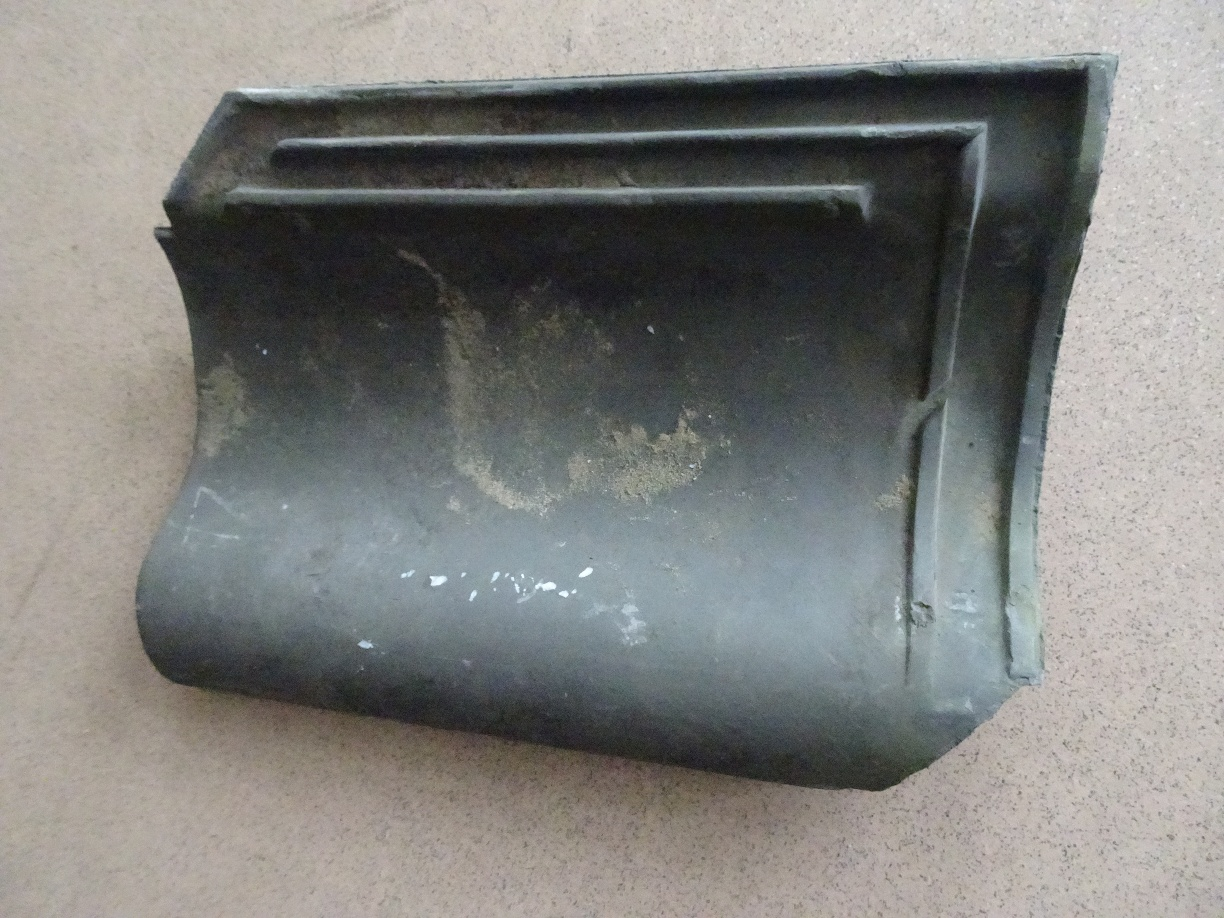
\includegraphics[width=\textwidth]{original.jpg}
% 		\caption{Original}
% 		\label{fig:original}
% 	\end{subfigure}
% 	\hfill
% 	\begin{subfigure}{0.45\textwidth}
% 		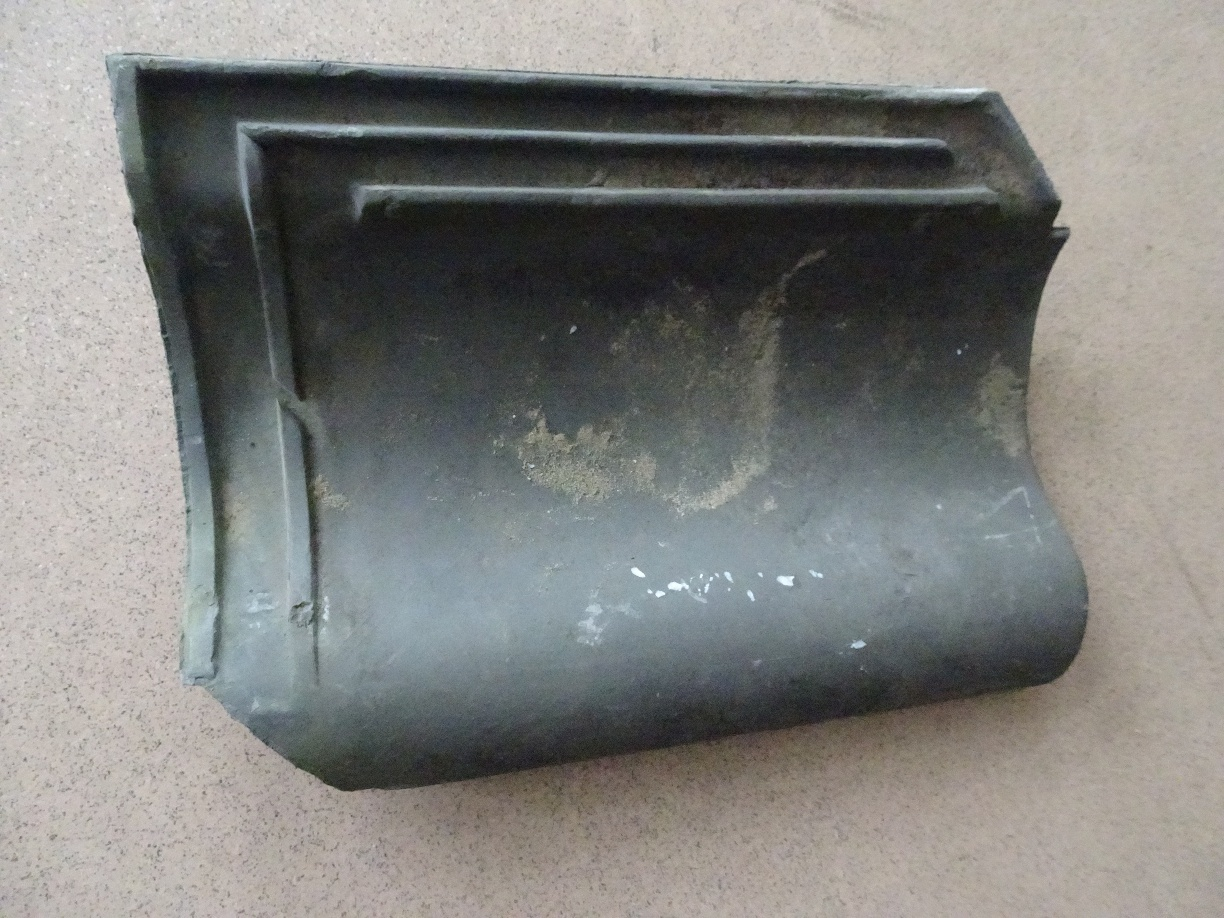
\includegraphics[width=\textwidth]{horizontal_flip.jpg}
% 		\caption{After augmentation}
% 		\label{fig:horizontal_flip}
% 	\end{subfigure}
% 	\label{fig:comparison}
% \end{figure}

\subsubsection{Rotation}
\begin{fullwidth}
	Wihin the realm of rotation, we will discuss multiple endpoints of a rotated image: $180^{\circ}$ and $90^{\circ}$. 
	All rotations will be done clockwise. 
\end{fullwidth}

\sidenote{$180^{\circ}$ rotation. A copy of the original image will be generated just for the trainingset.}

\begin{figure}[H]
	\centering
	\begin{subfigure}{0.45\textwidth}
		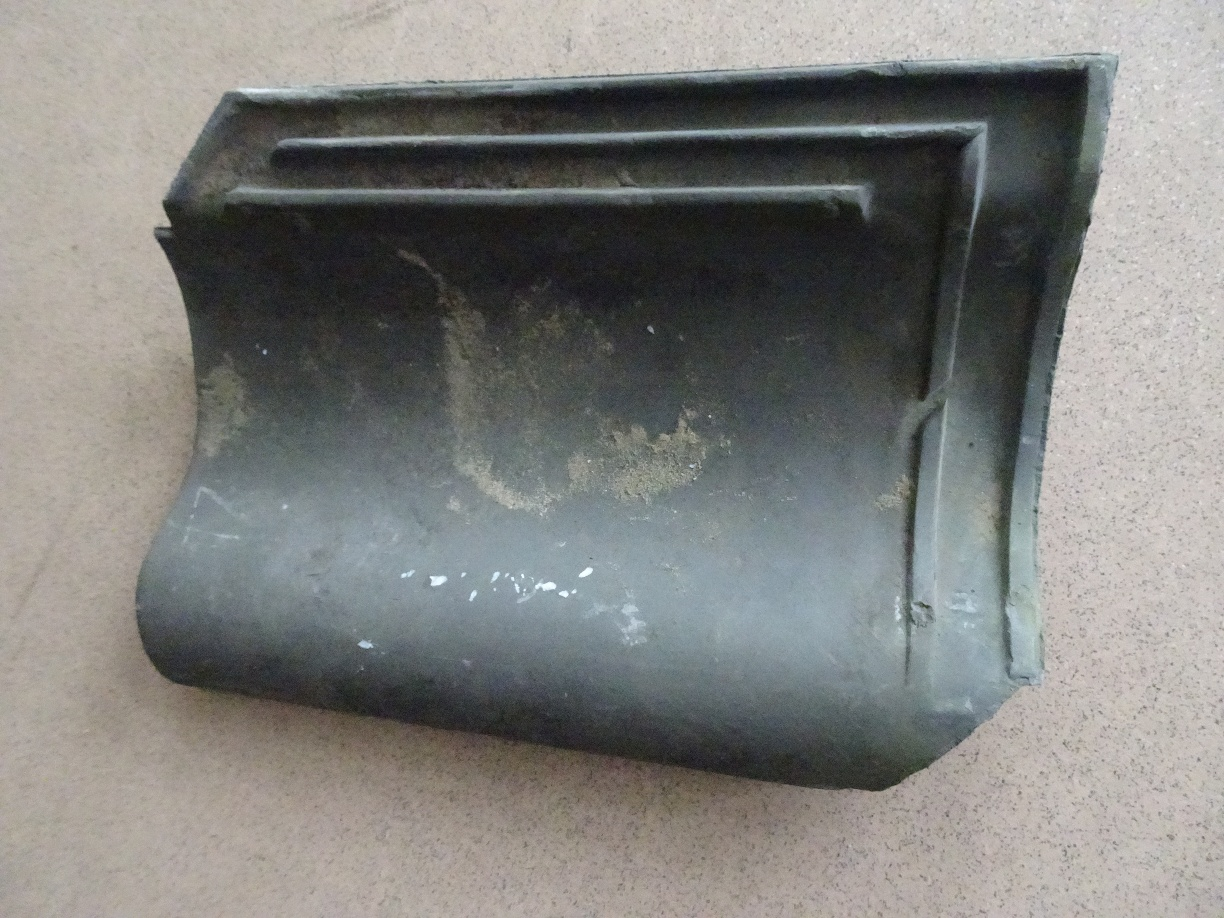
\includegraphics[width=\textwidth]{original.jpg}
		\caption{Original}
		\label{fig:original}
	\end{subfigure}
	\hfill
	\begin{subfigure}{0.45\textwidth}
		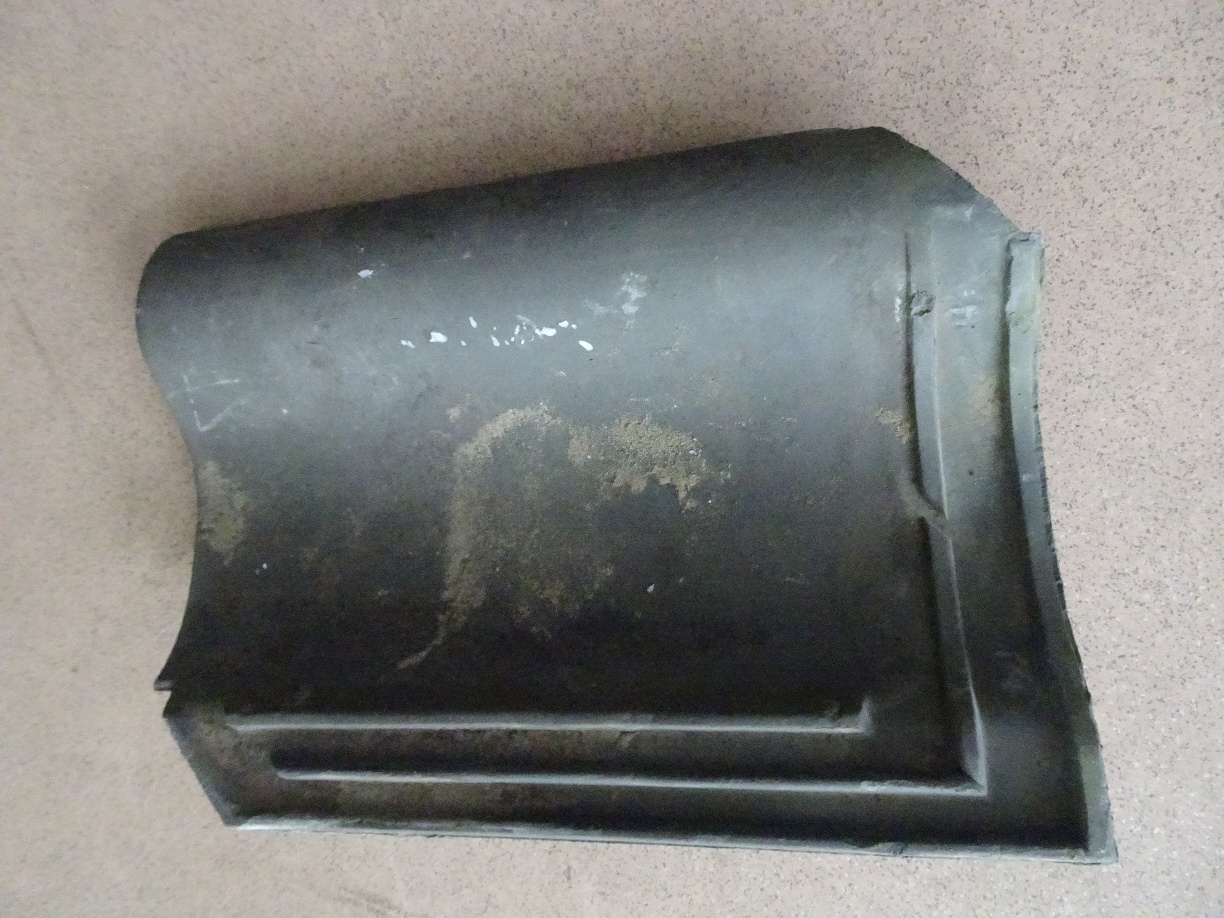
\includegraphics[width=\textwidth]{vertical_flip.jpg}
		\caption{After augmentation}
		\label{fig:vertical_flip}
	\end{subfigure}
	\label{fig:comparison}
\end{figure}

% \newpage
\sidenote{$90^{\circ}$ rotation. A copy of the original image will be generated just for the trainingset.}

\begin{figure}[H]
	\centering
	\begin{subfigure}{0.45\textwidth}
		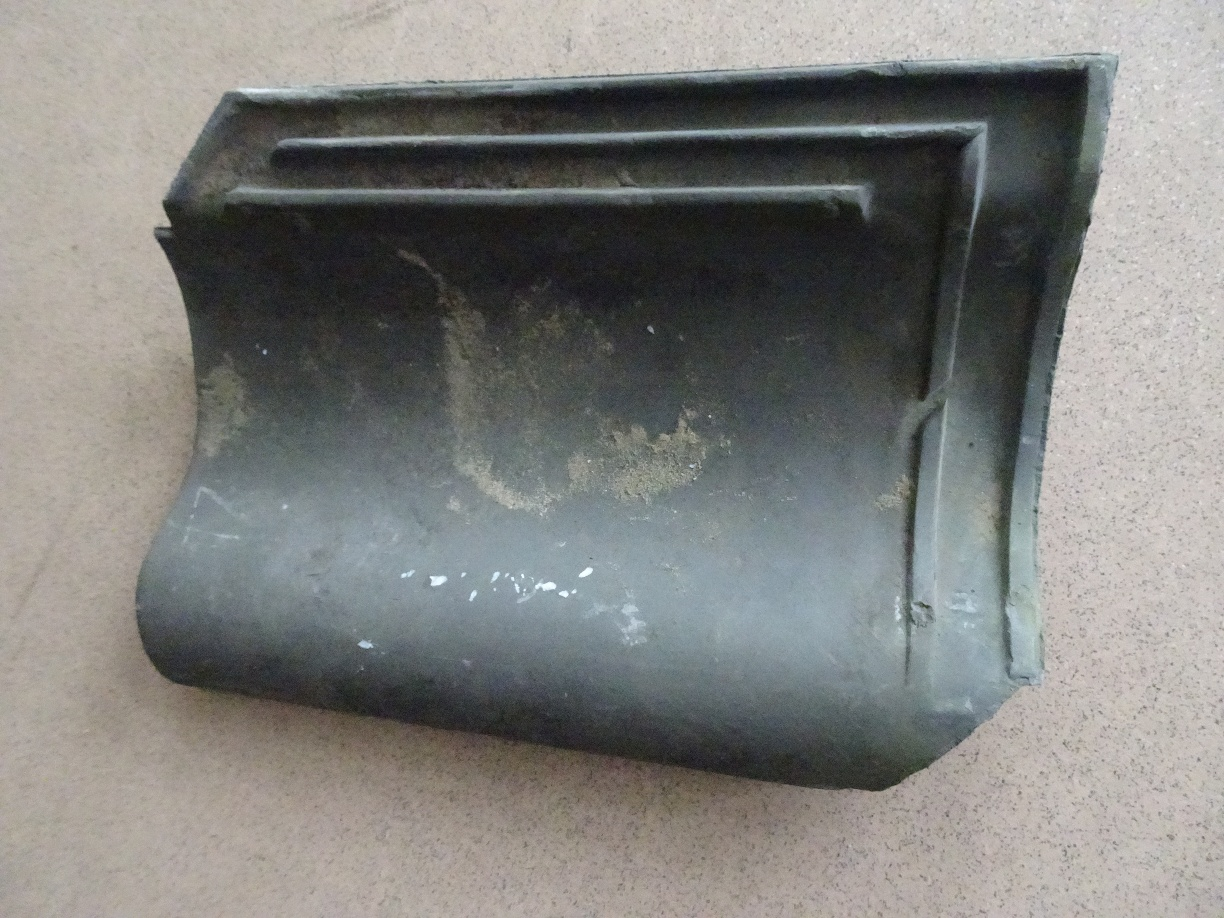
\includegraphics[width=\textwidth]{original.jpg}
		\caption{Original}
		\label{fig:original}
	\end{subfigure}
	\hfill
	\begin{subfigure}{0.45\textwidth}
		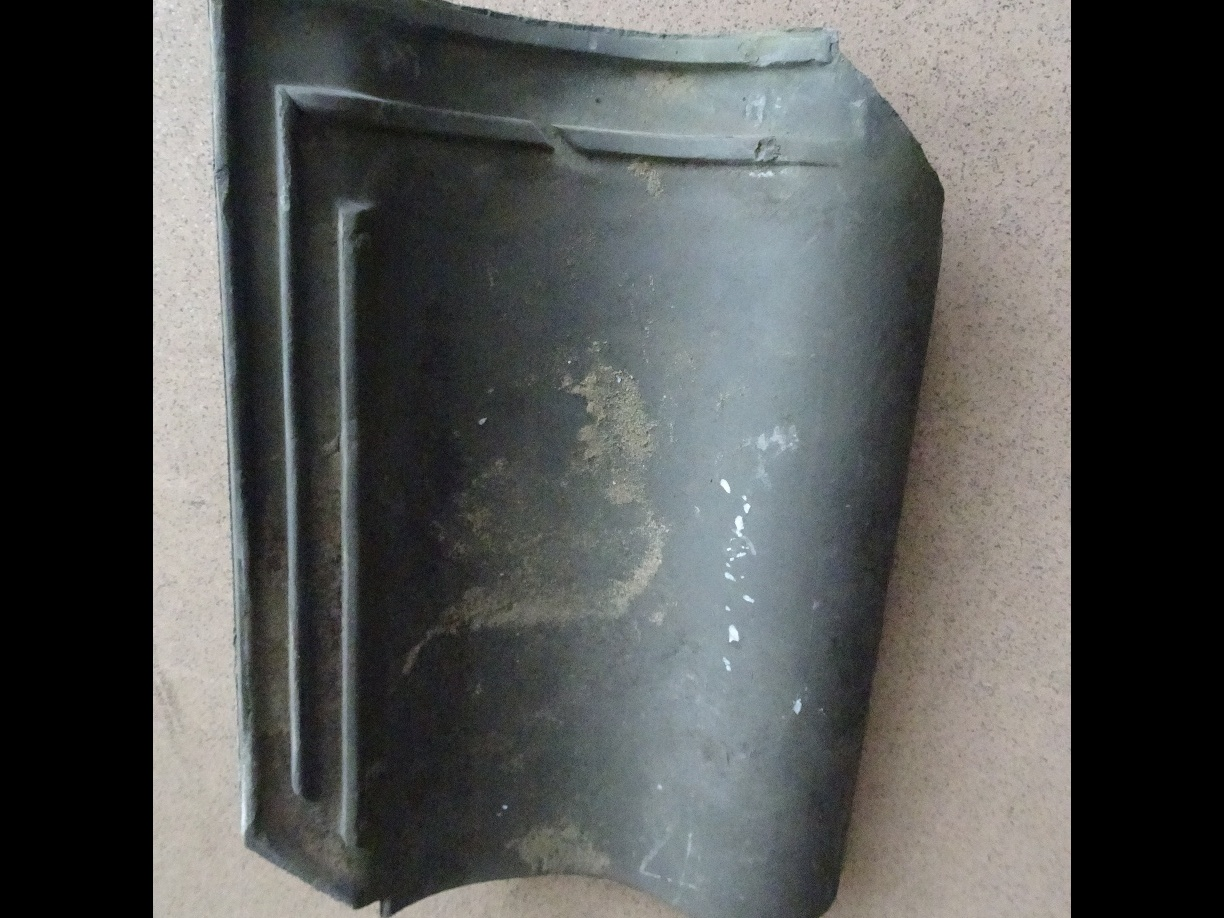
\includegraphics[width=\textwidth]{random_rotation.jpg}
		\caption{After augmentation}
		\label{fig:random_rotation}
	\end{subfigure}
	\label{fig:comparison}
\end{figure}

\newpage
\subsubsection{Zoom}
\sidenote{A copy of the original image from the dataset gets a zoomed version.
For better diversity there will be version of images that are zoomed in. 
This like the other methods is to increase diversity.}

\begin{figure}[H]
	\centering
	\begin{subfigure}{0.45\textwidth}
		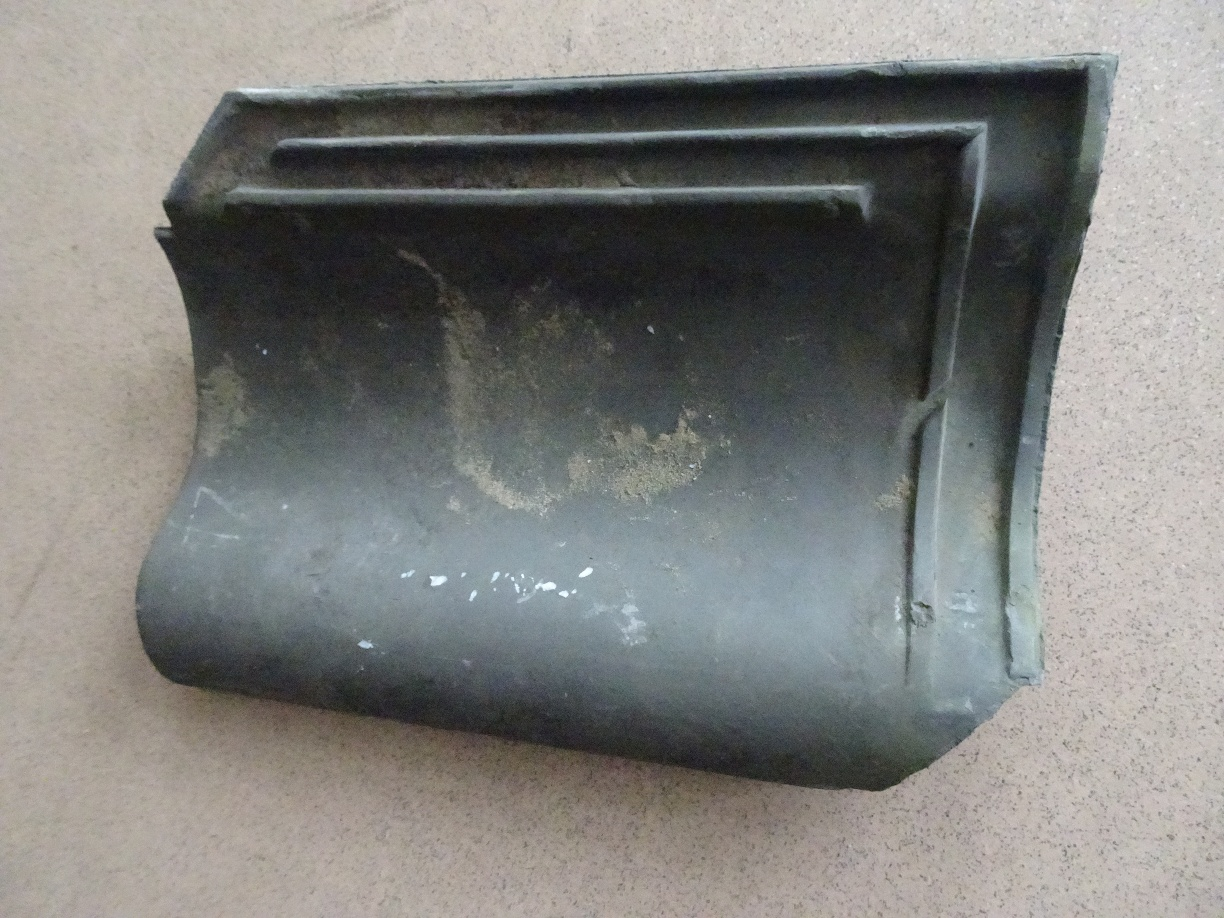
\includegraphics[width=\textwidth]{original.jpg}
		\caption{Original}
		\label{fig:original}
	\end{subfigure}
	\hfill
	\begin{subfigure}{0.45\textwidth}
		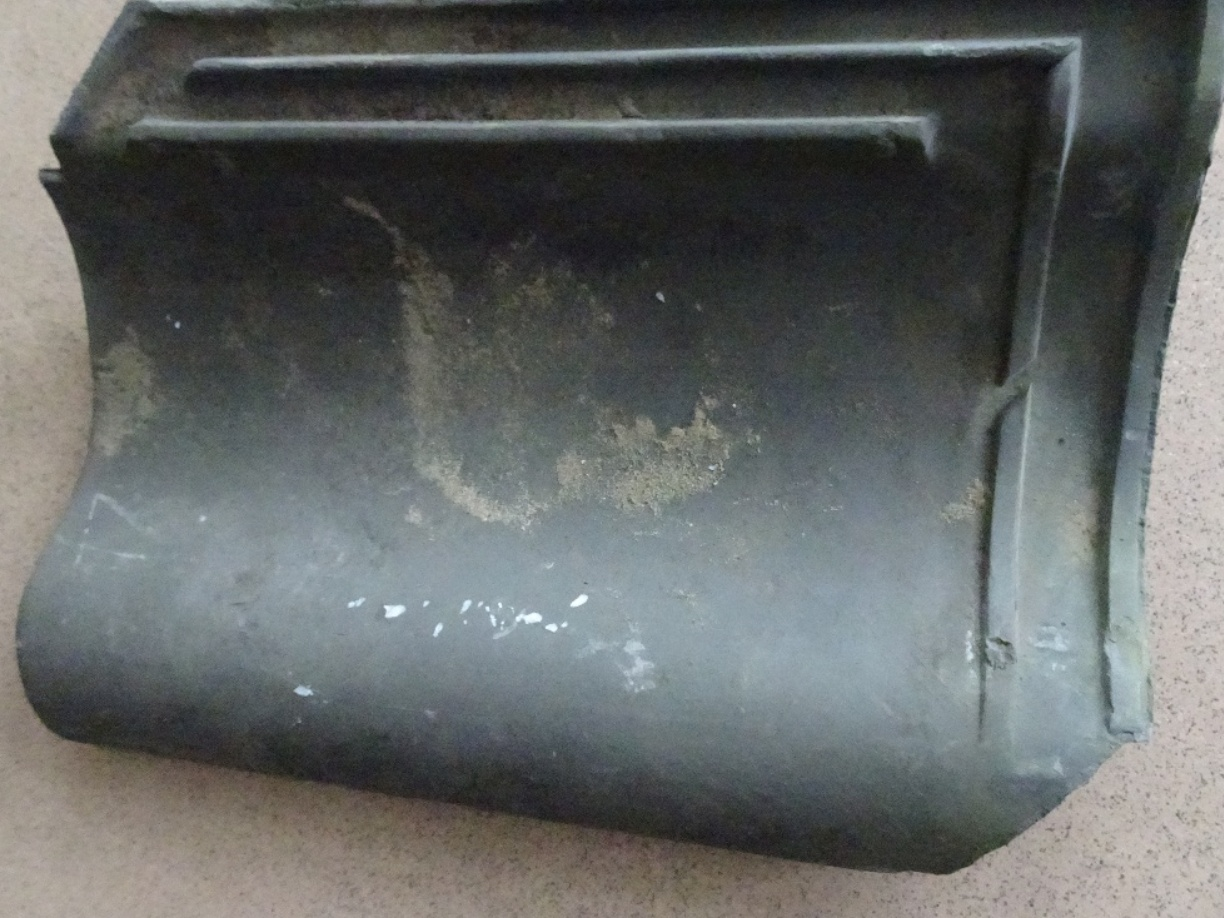
\includegraphics[width=\textwidth]{random_zoom.jpg}
		\caption{After augmentation}
		\label{fig:random_zoom}
	\end{subfigure}
	\label{fig:comparison}
\end{figure}



% Lorem ipsum dolor sit amet, consectetur adipiscing elit. Aliquam auctor mi risus, quis tempor libero hendrerit at. Duis hendrerit placerat quam et semper. Nam ultricies metus vehicula arcu viverra, vel ullamcorper justo elementum. Pellentesque vel mi ac lectus cursus posuere et nec ex. Fusce quis mauris egestas lacus commodo venenatis. Ut at arcu lectus. Donec et urna nunc. Morbi eu nisl cursus sapien eleifend tincidunt quis quis est. Donec ut orci ex. Praesent ligula enim, ullamcorper non lorem a, ultrices volutpat dolor. Nullam at imperdiet urna. Pellentesque nec velit eget est pretium.\sidenote{This is a sidenote. This template features a large margin specifically so you can put notes, figures, tables and other things into it as additional material to the main content in the text block.}

% Donec in elit ac ante vestibulum rhoncus. Pellentesque ligula tortor, aliquet malesuada nulla tristique vitae. Aliquam mi sem, varius eu pellentesque et, tristique nec quam. Vestibulum pellentesque in dui et venenatis. Sed malesuada elit pellentesque sapien aliquet porta. In at facilisis diam. Duis id ante tellus.\sidenote[][2cm]{This sidenote has been pushed down the page manually with an optional parameter, otherwise it would be right under the one above.} % This first optional argument to a sidenote is the symbol to use (leave this empty for automatic numbering) and the second is the vertical offset (positive is down, negative is up)

% \subsection{Subsection Title} % Second level section

% In diam libero, vulputate quis accumsan non, auctor in ipsum. Praesent cursus velit eget lacus sodales porta. Proin quis risus ut velit euismod scelerisque ut sed neque. Cras sagittis, dolor ac ullamcorper auctor, tortor dui facilisis diam, at sagittis nisi ipsum a neque. Nullam vel mattis nisi. Ut interdum ut diam at ornare. Nulla ultrices elit justo, vitae tristique massa vulputate sit amet.

% \nonumsidenote{This sidenote isn't numbered in the text or margin. This is useful for notes that apply anywhere on the page instead of one particular place.}Vestibulum erat felis, cursus vitae convallis ac, commodo eu nisi. Nulla facilisi. Mauris dignissim nisi felis, a mollis ex accumsan vel. Suspendisse bibendum vitae nibh in suscipit. Vestibulum et finibus eros. Nulla facilisi. Cras luctus aliquam finibus. In nec justo nec orci malesuada faucibus.

% \subsubsection{Subsubsection Title} % Third level section

% \begin{fullwidth} % Use the whole page width
% 	\textit{This is an example of a full width paragraph\ldots} Curabitur id placerat orci. Vivamus pulvinar augue ac feugiat blandit. Donec in ultricies mi. Nam eu lacus ac augue aliquet consectetur. Praesent dui risus, sollicitudin nec felis ut, posuere ultricies dolor. Sed massa nulla, dignissim eget sem sit amet, eleifend fermentum dui. Phasellus consequat sem vel turpis finibus, a aliquam risus malesuada.
% \end{fullwidth}

% Maecenas consectetur metus at tellus finibus condimentum. Proin arcu lectus, ultrices non tincidunt et, tincidunt ut quam. Integer luctus posuere est, non maximus ante dignissim quis. Nunc a cursus erat. Curabitur suscipit nibh in tincidunt sagittis. Nam malesuada vestibulum quam id gravida. Proin ut dapibus velit. Vestibulum eget quam quis ipsum semper convallis. Duis consectetur nibh ac diam dignissim, id condimentum enim dictum. Nam aliquet ligula eu magna pellentesque, nec sagittis leo lobortis. Aenean tincidunt dignissim egestas. Morbi efficitur risus ante, id tincidunt odio pulvinar vitae.

% \paragraph{Paragraph Title} % Fourth level section

% Lorem ipsum dolor sit amet, consectetur adipiscing elit. Aliquam auctor mi risus, quis tempor libero hendrerit at. Duis hendrerit placerat quam et semper. Nam ultricies metus vehicula arcu viverra, vel ullamcorper justo elementum. Pellentesque vel mi ac lectus cursus posuere et nec ex.

% The section titles below show how multi-line section titles look at the 3 top levels.

% \section[Short version of long section title]{Fusce eleifend porttitor arcu, id accumsan elit pharetra eget} % Use the optional parameter to the \section command to specify a shorter version of the title for the table of contents

% Lorem ipsum dolor sit amet, consectetur adipiscing elit. \nonumsidenote[-2cm]{Section, subsection and subsubsection titles can span multiple lines, as shown here. Make sure to put a shorter version of these long titles in the optional parameter to the section commands so the title output to the table of contents is the short version.}

% \subsection[Short version of long subsection title]{Phasellus sit amet enim efficitur, aliquam nulla id, lacinia mauris viverra libero ac magna}

% Lorem ipsum dolor sit amet, consectetur adipiscing elit.

% \subsubsection{In mi mauris, finibus non faucibus non, imperdiet nec leo. In erat arcu, tincidunt nec aliquam et, volutpat eget}

% Lorem ipsum dolor sit amet, consectetur adipiscing elit.

%----------------------------------------------------------------------------------------
%	FIGURES
%----------------------------------------------------------------------------------------

% \section{Figure Examples}

% This statement automatically references the figure below using its label: Figure \ref{fig:example}.

%------------------------------------------------

% \begin{marginfigure} % Use the marginfigure environment for figures to be output to the margin
% 	
\includegraphics[width=\linewidth]{placeholder.jpg}
% 	\caption{Margin figure caption.}
% \end{marginfigure}

% %------------------------------------------------

% \begin{figure}[H] % [H] forces the figure to be output where it is defined in the code (it suppresses floating)
% 	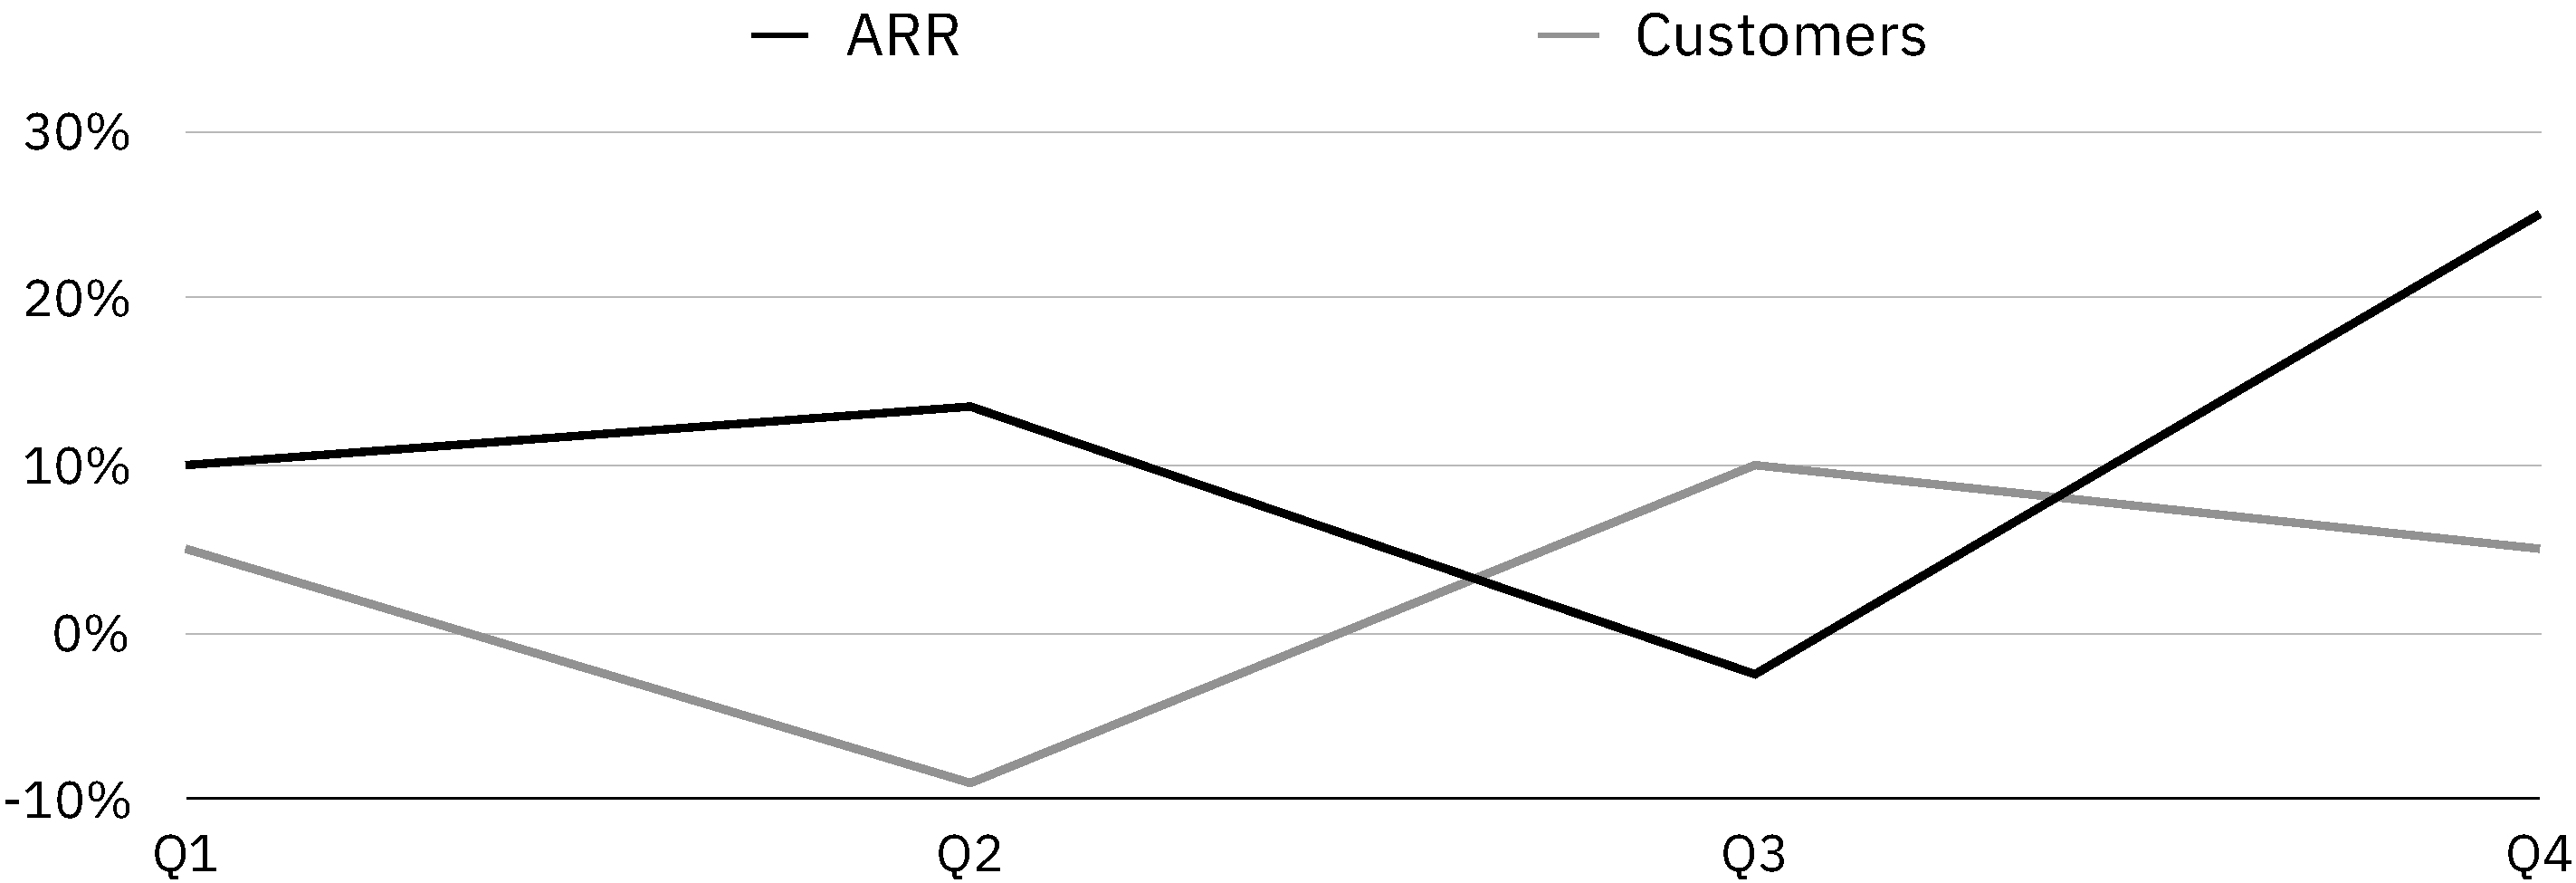
\includegraphics[width=\linewidth]{ARR.pdf}
% 	\caption{Text block figure caption.}
% 	\label{fig:example} % Label for referencing this figure in the text automatically
% \end{figure}

% %------------------------------------------------

% \begin{figure*} % Use the figure* environment for full width figures
% 	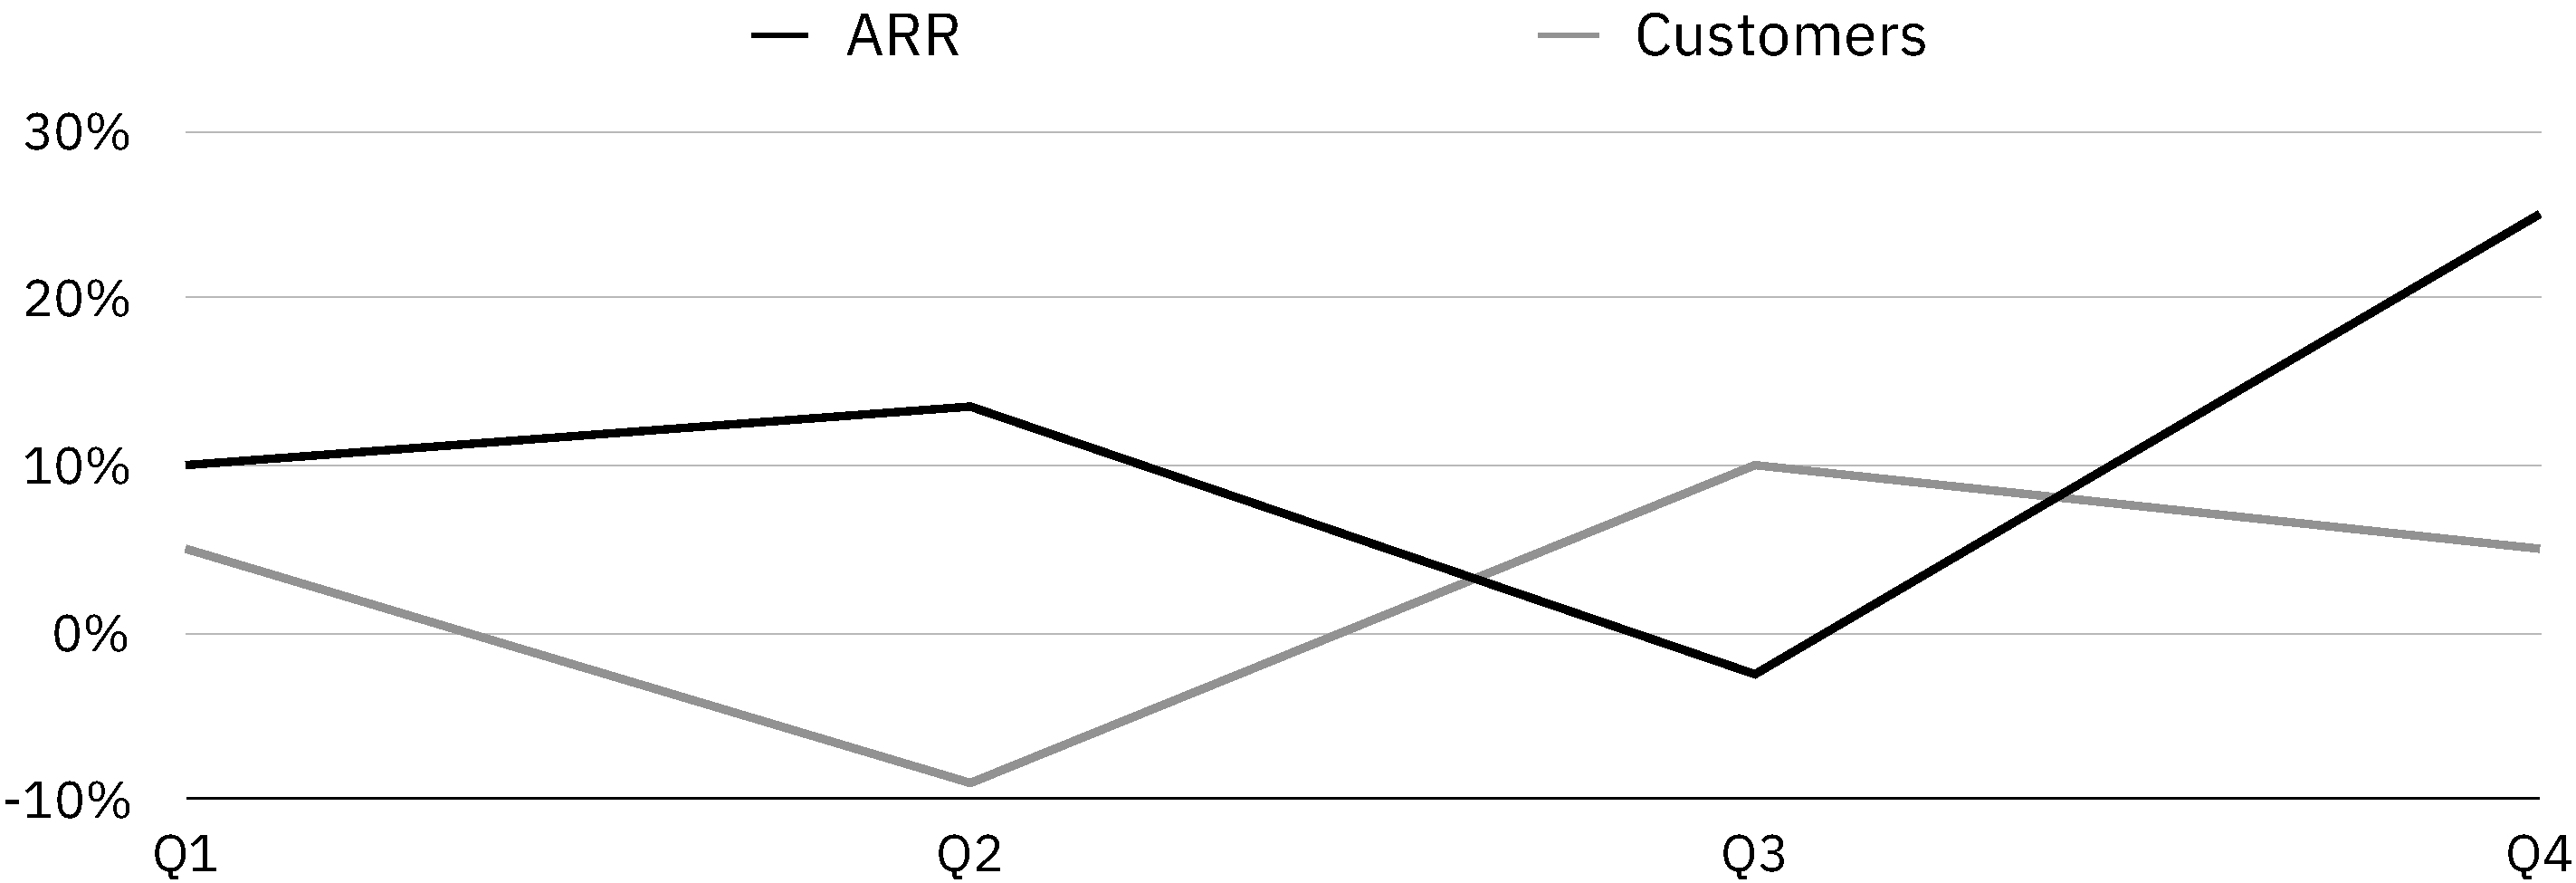
\includegraphics[width=\linewidth]{ARR.pdf}
% 	\caption{Full width figure caption.}
% \end{figure*}

%----------------------------------------------------------------------------------------


\end{document}
